% !TeX root = ../main.tex
\chapter{XÂY DỰNG HỆ THỐNG}
\section{Phân tích yêu cầu}

\subsection{Sơ đồ usecase chính}


\begin{figure}[h]
	\centering
	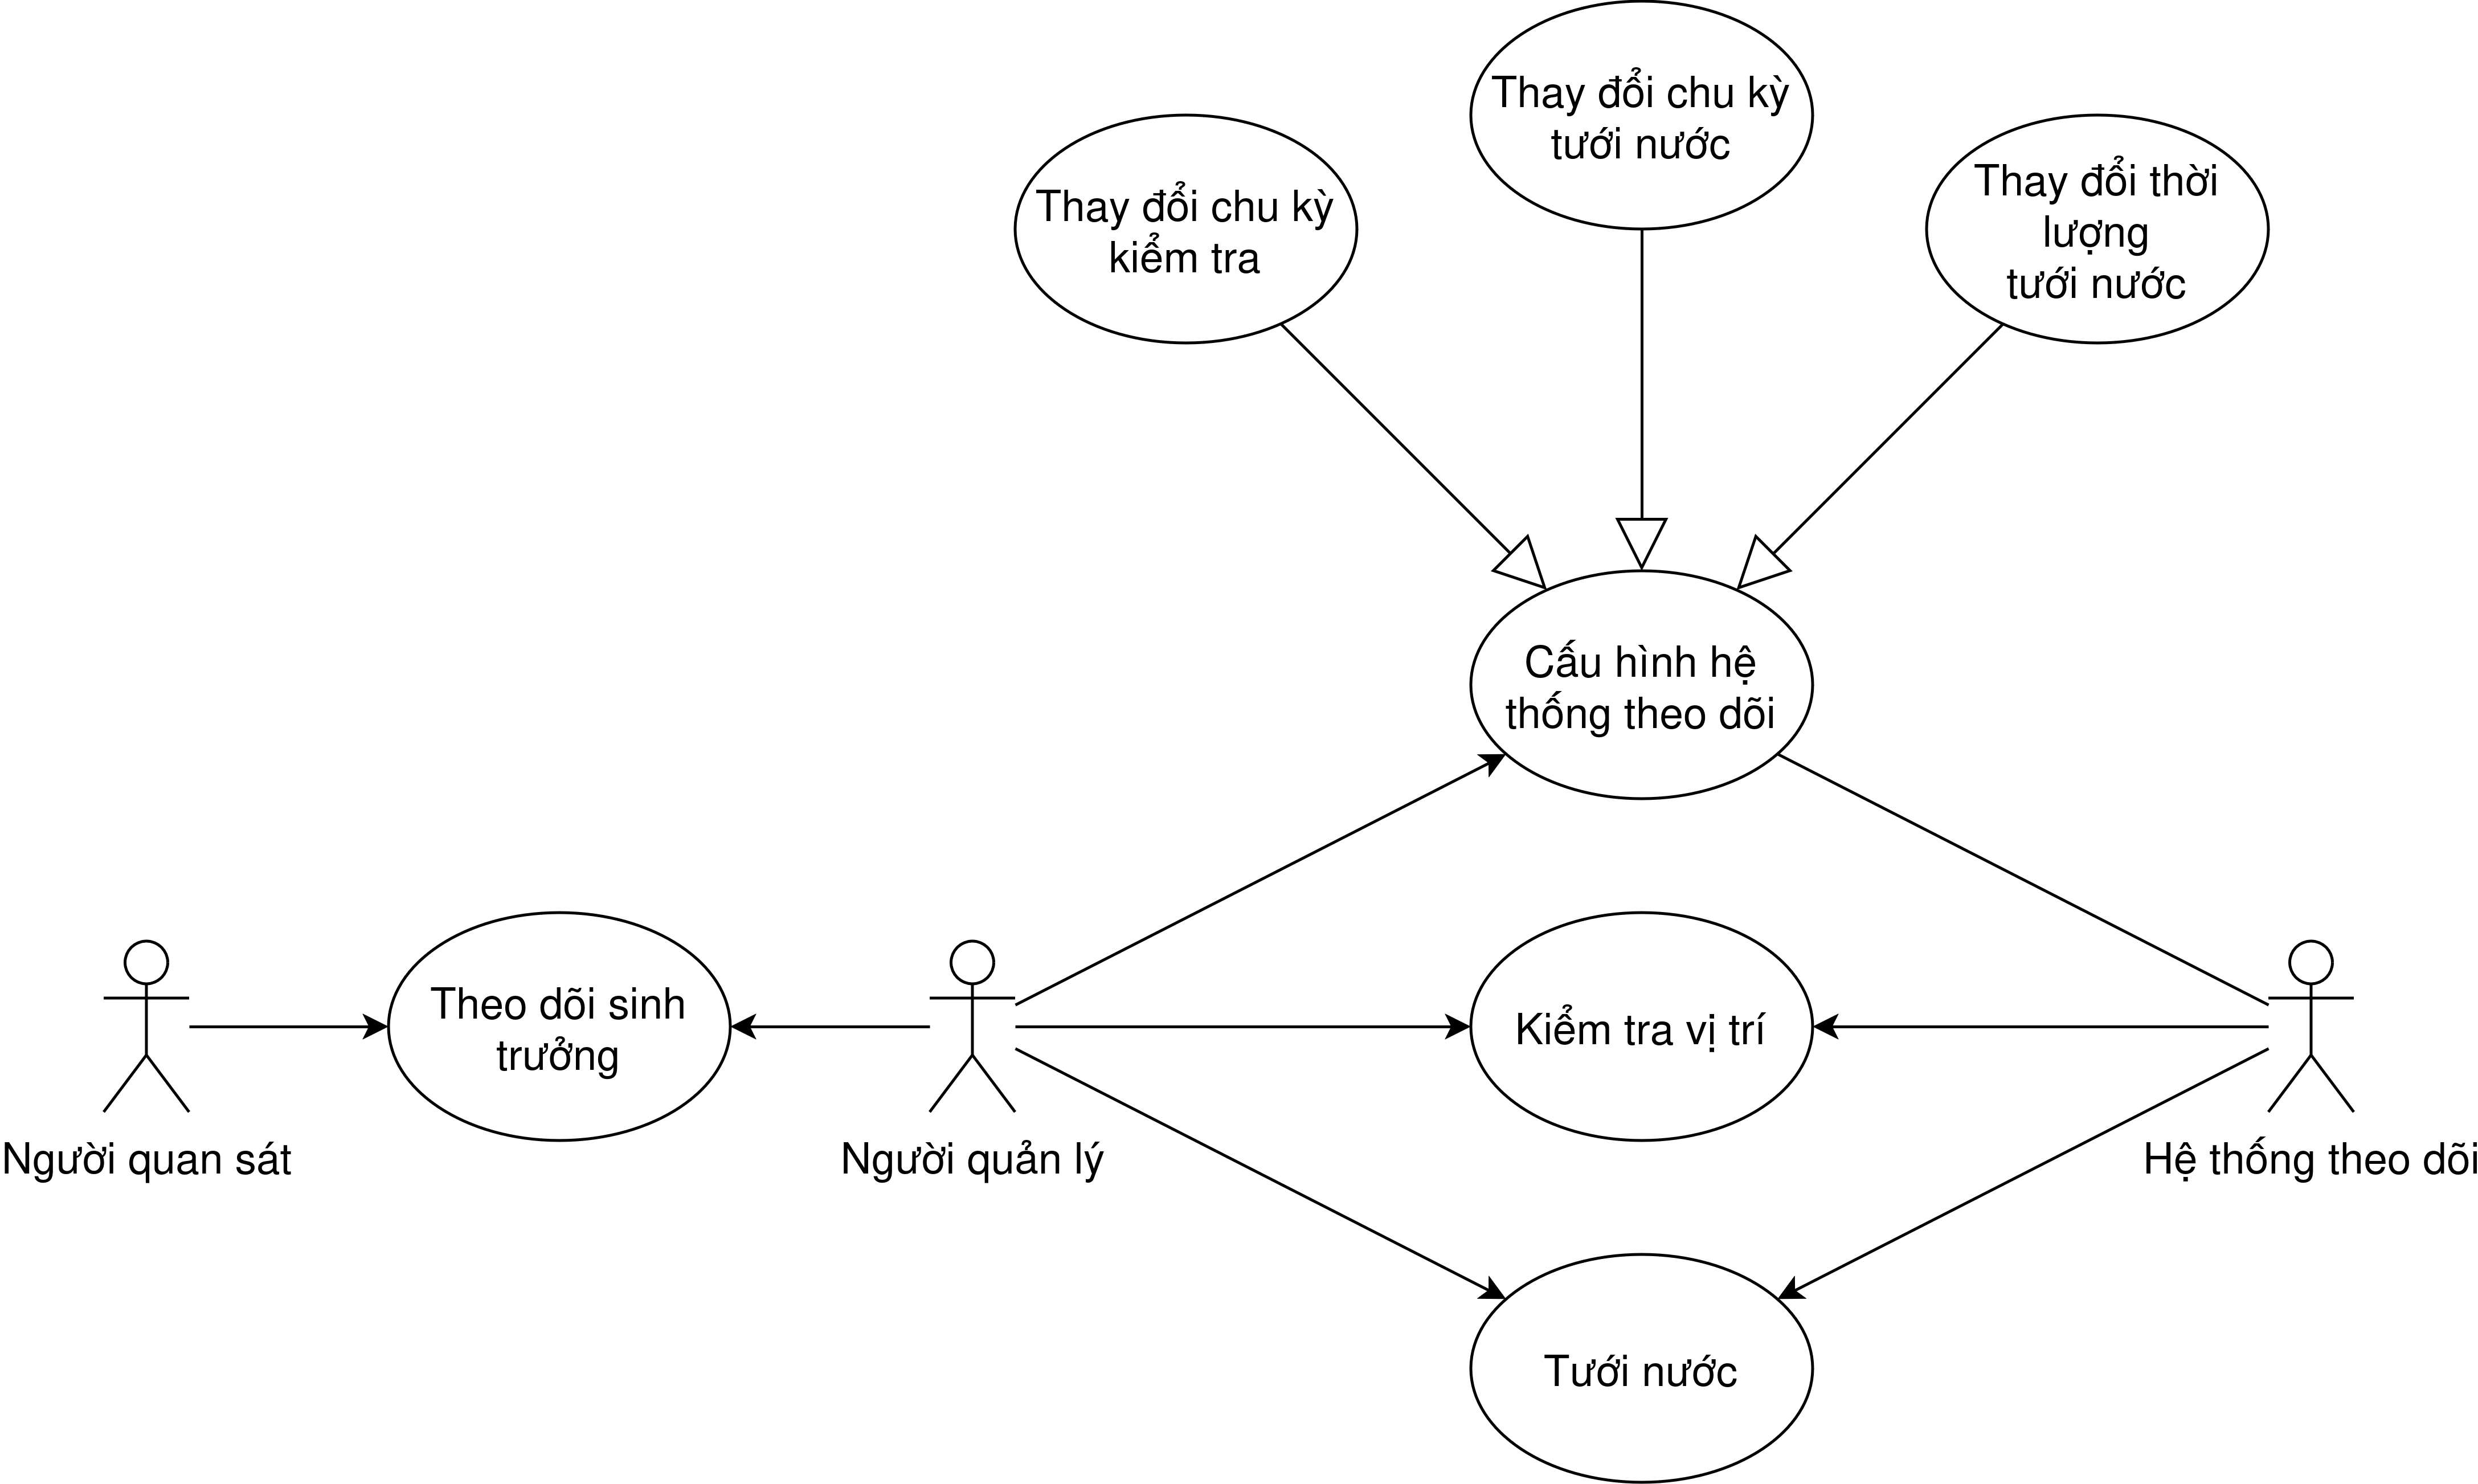
\includegraphics[width=\linewidth]{images/main-usecase}
	\caption{Usecase chính}
	\label{fig:main-usecase}
\end{figure}

\subsubsection{Đặc tả usecase tưới nước}

% Please add the following required packages to your document preamble:
% \usepackage{longtable}
% Note: It may be necessary to compile the document several times to get a multi-page table to line up properly
\begin{longtable}[c]{|l|p{11cm}|}
	\caption{Đặc tả usecase tưới nước}
	\label{tab:des-water}\\
	\hline
	\textbf{Usecase} & \textbf{Nội dung}                                                                                  \\ \hline
	\endfirsthead
	\hline
	\textbf{Usecase} & \textbf{Nội dung}                                                                                  \\ \hline
	\endhead
	%
	Tên usecase      & Tưới nước                                                                                          \\ \hline
	Mô tả               & Cho phép người quản lý hoặc hệ thống tưới nước tại vị trí chỉ định.                                \\ \hline
	Người dùng          & Người quản lý, hệ thống theo dõi tự động.                                                          \\ \hline
	Điều kiện kích hoạt & Khi người quản lý muốn thực hiện tưới nước thủ công hoặc tự động tưới sau một khoảng thời gian đặt sẵn. \\ \hline
	Tiền điều kiện      & Người quản lý đăng nhập thành công vào hệ thống.                                                   \\ \hline
	Hậu điều kiện       & Vị trí phôi nấm được tưới nước và ghi nhận vào hệ thống.                                           \\ \hline
	Luồng sự kiện chính &
	\begin{tabular}[c]{p{10.5cm}}1. Người quản lý truy cập trang “Dashboard”.\\ 2. Người quản lý chọn thẻ tương ứng với phôi nấm muốn tưới.\\ 3. Người quản lý nhấn “Water”.\\ 4. Hệ thống thực hiện di chuyển tới vị trí tưới nấm, kiểm tra và tươi nấm.\\ 5. Hệ thống hiển thị hình ảnh tưới nấm và cập nhật lại trang.\end{tabular} \\ \hline
	Luồng sự kiện thay thế &
	\begin{tabular}[c]{p{10.5cm}}
		\textbf{- Hoạt động tưới bởi hệ thống theo dõi tự động:}\\
		1. Hệ thống theo dõi kiểm tra vị trí nấm theo chu kỳ kiểm tra được cài đặt sẵn.\\
		2. Khi lần tưới trước xảy ra vượt quá chu kỳ tưới nước, thực hiện di chuyển, kiểm tra và tưới nấm theo cài đặt.\\
		\textbf{- Tưới nước theo từng trạng thái phát triển:}\\
		1. Người quản lý truy cập trang "Dashboard"\\
		2. Người quản lý chọn trạng thái phát triển tương ứng trong bảng điều khiển\\
		3. Hệ thống lọc các vị trí phù hợp với trạng thái được chọn và hiển thị lên bảng điều khiển.\\
		4. Người dùng nhấn "Water All"\\
		5. Hệ thống di chuyển tới từng vị trí tương ứng và kiểm tra, tưới nấm
	\end{tabular} \\ \hline
\end{longtable}

\subsubsection{Đặc tả usecase kiểm tra vị trí}

% Please add the following required packages to your document preamble:
% \usepackage{longtable}
% Note: It may be necessary to compile the document several times to get a multi-page table to line up properly
\begin{longtable}[c]{|l|p{11cm}|}
	\caption{Đặc tả usecase kiểm tra vị trí}
	\label{tab:des-check}\\
	\hline
	\textbf{Usecase} & \textbf{Nội dung}                                                                                  \\ \hline
	\endfirsthead
	\hline
	\textbf{Usecase} & \textbf{Nội dung}                                                                                  \\ \hline
	\endhead
	%
	Tên usecase      & Kiểm tra vị trí                                                                                         \\ \hline
	Mô tả               & Cho phép người quản lý hoặc hệ thống kiểm tra trạng thái của vị trí chỉ định.                                \\ \hline
	Người dùng          & Người quản lý, hệ thống theo dõi tự động.                                                          \\ \hline
	Điều kiện kích hoạt & Khi người quản lý muốn thực hiện kiểm tra thủ công hoặc tự động kiểm tra sau một khoảng thời gian đặt sẵn. \\ \hline
	Tiền điều kiện      & Người quản lý đăng nhập thành công vào hệ thống.                                                   \\ \hline
	Hậu điều kiện       & Vị trí phôi nấm được tưới nước và ghi nhận vào hệ thống.                                           \\ \hline
	Luồng sự kiện chính &
	\begin{tabular}[c]{p{10.5cm}}
		1. Người quản lý truy cập trang “Dashboard”.\\
		2. Người quản lý chọn thẻ tương ứng với phôi nấm muốn tưới.\\
		3. Người quản lý nhấn “Check”.\\
		4. Hệ thống thực hiện di chuyển tới vị trí tưới nấm, kiểm tra và tươi nấm nếu tới chu kỳ tưới.\\
		5. Hệ thống hiển thị hình ảnh tưới nấm và cập nhật lại trang.
	\end{tabular} \\ \hline
	Luồng sự kiện thay thế &
	\begin{tabular}[c]{p{10.5cm}}
		\textbf{- Hoạt động tưới bởi hệ thống theo dõi tự động}\\
		1. Hệ thống theo dõi kiểm tra vị trí nấm theo chu kỳ kiểm tra được cài đặt sẵn.\\
		2. Khi lần kiểm tra trước xảy ra vượt quá chu kỳ kiểm tra, thực hiện di chuyển, kiểm tra và tưới nấm nếu đạt điều kiện theo cài đặt.\\
		\textbf{- Kiểm tra theo từng trạng thái phát triển:}\\
		1. Người quản lý truy cập trang "Dashboard"\\
		2. Người quản lý chọn trạng thái phát triển tương ứng trong bảng điều khiển\\
		3. Hệ thống lọc các vị trí phù hợp với trạng thái được chọn và hiển thị lên bảng điều khiển.\\
		4. Người dùng nhấn "Check All"\\
		5. Hệ thống di chuyển tới từng vị trí tương ứng, kiểm tra và tưới nấm nếu thỏa mãn điều kiện tưới tự động.
	\end{tabular} \\ \hline
\end{longtable}

\subsubsection{Đặc tả usecase cấu hình hệ thống theo dõi}
% Please add the following required packages to your document preamble:
% \usepackage{longtable}
% Note: It may be necessary to compile the document several times to get a multi-page table to line up properly
\begin{longtable}[c]{|l|p{11cm}|}
	\caption{Đặc tả usecase ucấu hình hệ thống theo dõi}
	\label{tab:des-stage-config}\\
	\hline
	\textbf{Usecase} & \textbf{Nội dung}                                                                                  \\ \hline
	\endfirsthead
	\hline
	\textbf{Usecase}    & \textbf{Nội dung}                                                                                              \\ \hline
	\endhead
	%
	Tên usecase         & Cấu hình hệ thống theo dõi.                                                                                    \\ \hline
	Mô tả                  & Cho phép người quản lý cấu hình hoạt động của hệ thống theo dõi tự động cho từng giai đoạn phát triển của nấm. \\ \hline
	Người dùng             & Người quản lý.                                                                                                 \\ \hline
	Điều kiện kích hoạt    & Khi người quản lý muốn cấu hình hệ thống theo dõi tự động theo chu kỳ đặt sẵn.                                 \\ \hline
	Tiền điều kiện         & Người quản lý đăng nhập thành công vào hệ thống.                                                               \\ \hline
	Hậu điều kiện          & Hệ thống theo dõi tự động được cấu hình thành công và hoạt động theo cấu hình mới                              \\ \hline
	Luồng sự kiện chính &
	\begin{tabular}[c]{p{10.5cm}}1. Người quản lý truy cập trang “Stage Management”.\\ 2. Người quản lý nhập giá trị “chu kỳ kiểm tra”, “chu kỳ tưới nước” và “thời lượng tưới” cho một giai đoạn phát triển và nhấn “Update”.\\ 3. Hệ thống ghi nhận giá trị cấu hình mới và cập nhật lại trang.\end{tabular} \\ \hline
	Luồng sự kiện thay thế & Không                                                                                                          \\ \hline
\end{longtable}

\subsubsection{Đặc tả usecase theo dõi sinh trưởng}

\begin{longtable}[c]{|l|p{11cm}|}
	\caption{Đặc tả usecase theo dõi sinh trưởng}
	\label{tab:des-monitor}\\
	\hline
	\textbf{Usecase} & \textbf{Nội dung}                                                                                  \\ \hline
	\endfirsthead
	\hline
	\textbf{Usecase}    & \textbf{Nội dung}                                                                                              \\ \hline
	\endhead
	%
	Tên usecase         & Theo dõi sinh trưởng.              \\ \hline
	Mô tả                  & Cho phép người quản lý hoặc người quan sát theo dõi sự phát triển của nấm qua thời gian tại vị trí được chọn. \\ \hline
	Người dùng             & Người quản lý, người quan sát. \\ \hline
	Điều kiện kích hoạt    & Khi người quản lý hoặc người quan sát muốn theo dõi sự phát triển của nấm tại các vị trí xác định.                                 \\ \hline
	Tiền điều kiện         & Người quản lý hoặc người quan sát đăng nhập thành công vào hệ thống.                                                               \\ \hline
	Hậu điều kiện          & Hệ thống hiển thị giao diện quản lý cho các vị trí được chỉ định.                              \\ \hline
	Luồng sự kiện chính &
	\begin{tabular}[c]{p{10.5cm}}
		1. Người quản lý hoặc người quan sát truy cập trang “Dashboard”.\\ 
		2. Hệ thống hiển thị các vị trí nấm và hình ảnh của lần kiểm tra gần nhất của từng vị trí.
	\end{tabular} \\ \hline
	Luồng sự kiện thay thế & 	\begin{tabular}[c]{p{10.5cm}}
		\textbf{- Lọc hiển thị từng trạng thái phát triển}\\
		1. Người quản lý hoặc người quan sát truy cập trang “Dashboard”.\\ 
		2. Hệ thống hiển thị các vị trí nấm và hình ảnh của lần kiểm tra gần nhất của từng vị trí.\\
		3. Người quản lý hoặc người quan sát chọn trạng thái sinh trưởng tương ứng trên bảng điều khiển.\\
		4. Hệ thống lọc các vị trí thỏa mãn và hiển thị trên bảng điều khiển.m\\
		\textbf{- Hiển thị một vị trí xác dịnh}\\
		1. Người quản lý hoặc người quan sát truy cập trang “Dashboard”.\\ 
		2. Hệ thống hiển thị các vị trí nấm và hình ảnh của lần kiểm tra gần nhất của từng vị trí.\\
		3. Người quản lý hoặc người quan sát nhấn vào hình ảnh hoặc vị trí tương ứng trong danh sách vị trí.\\
		4. Hệ thống hiển thị chi tiết thông tin của vị trí cùng lịch sử kiểm tra, tưới nước.
	\end{tabular} \\ \hline
\end{longtable}

\subsection{Sơ đồ usecase cho người quản trị}

\begin{figure}[H]
	\centering
	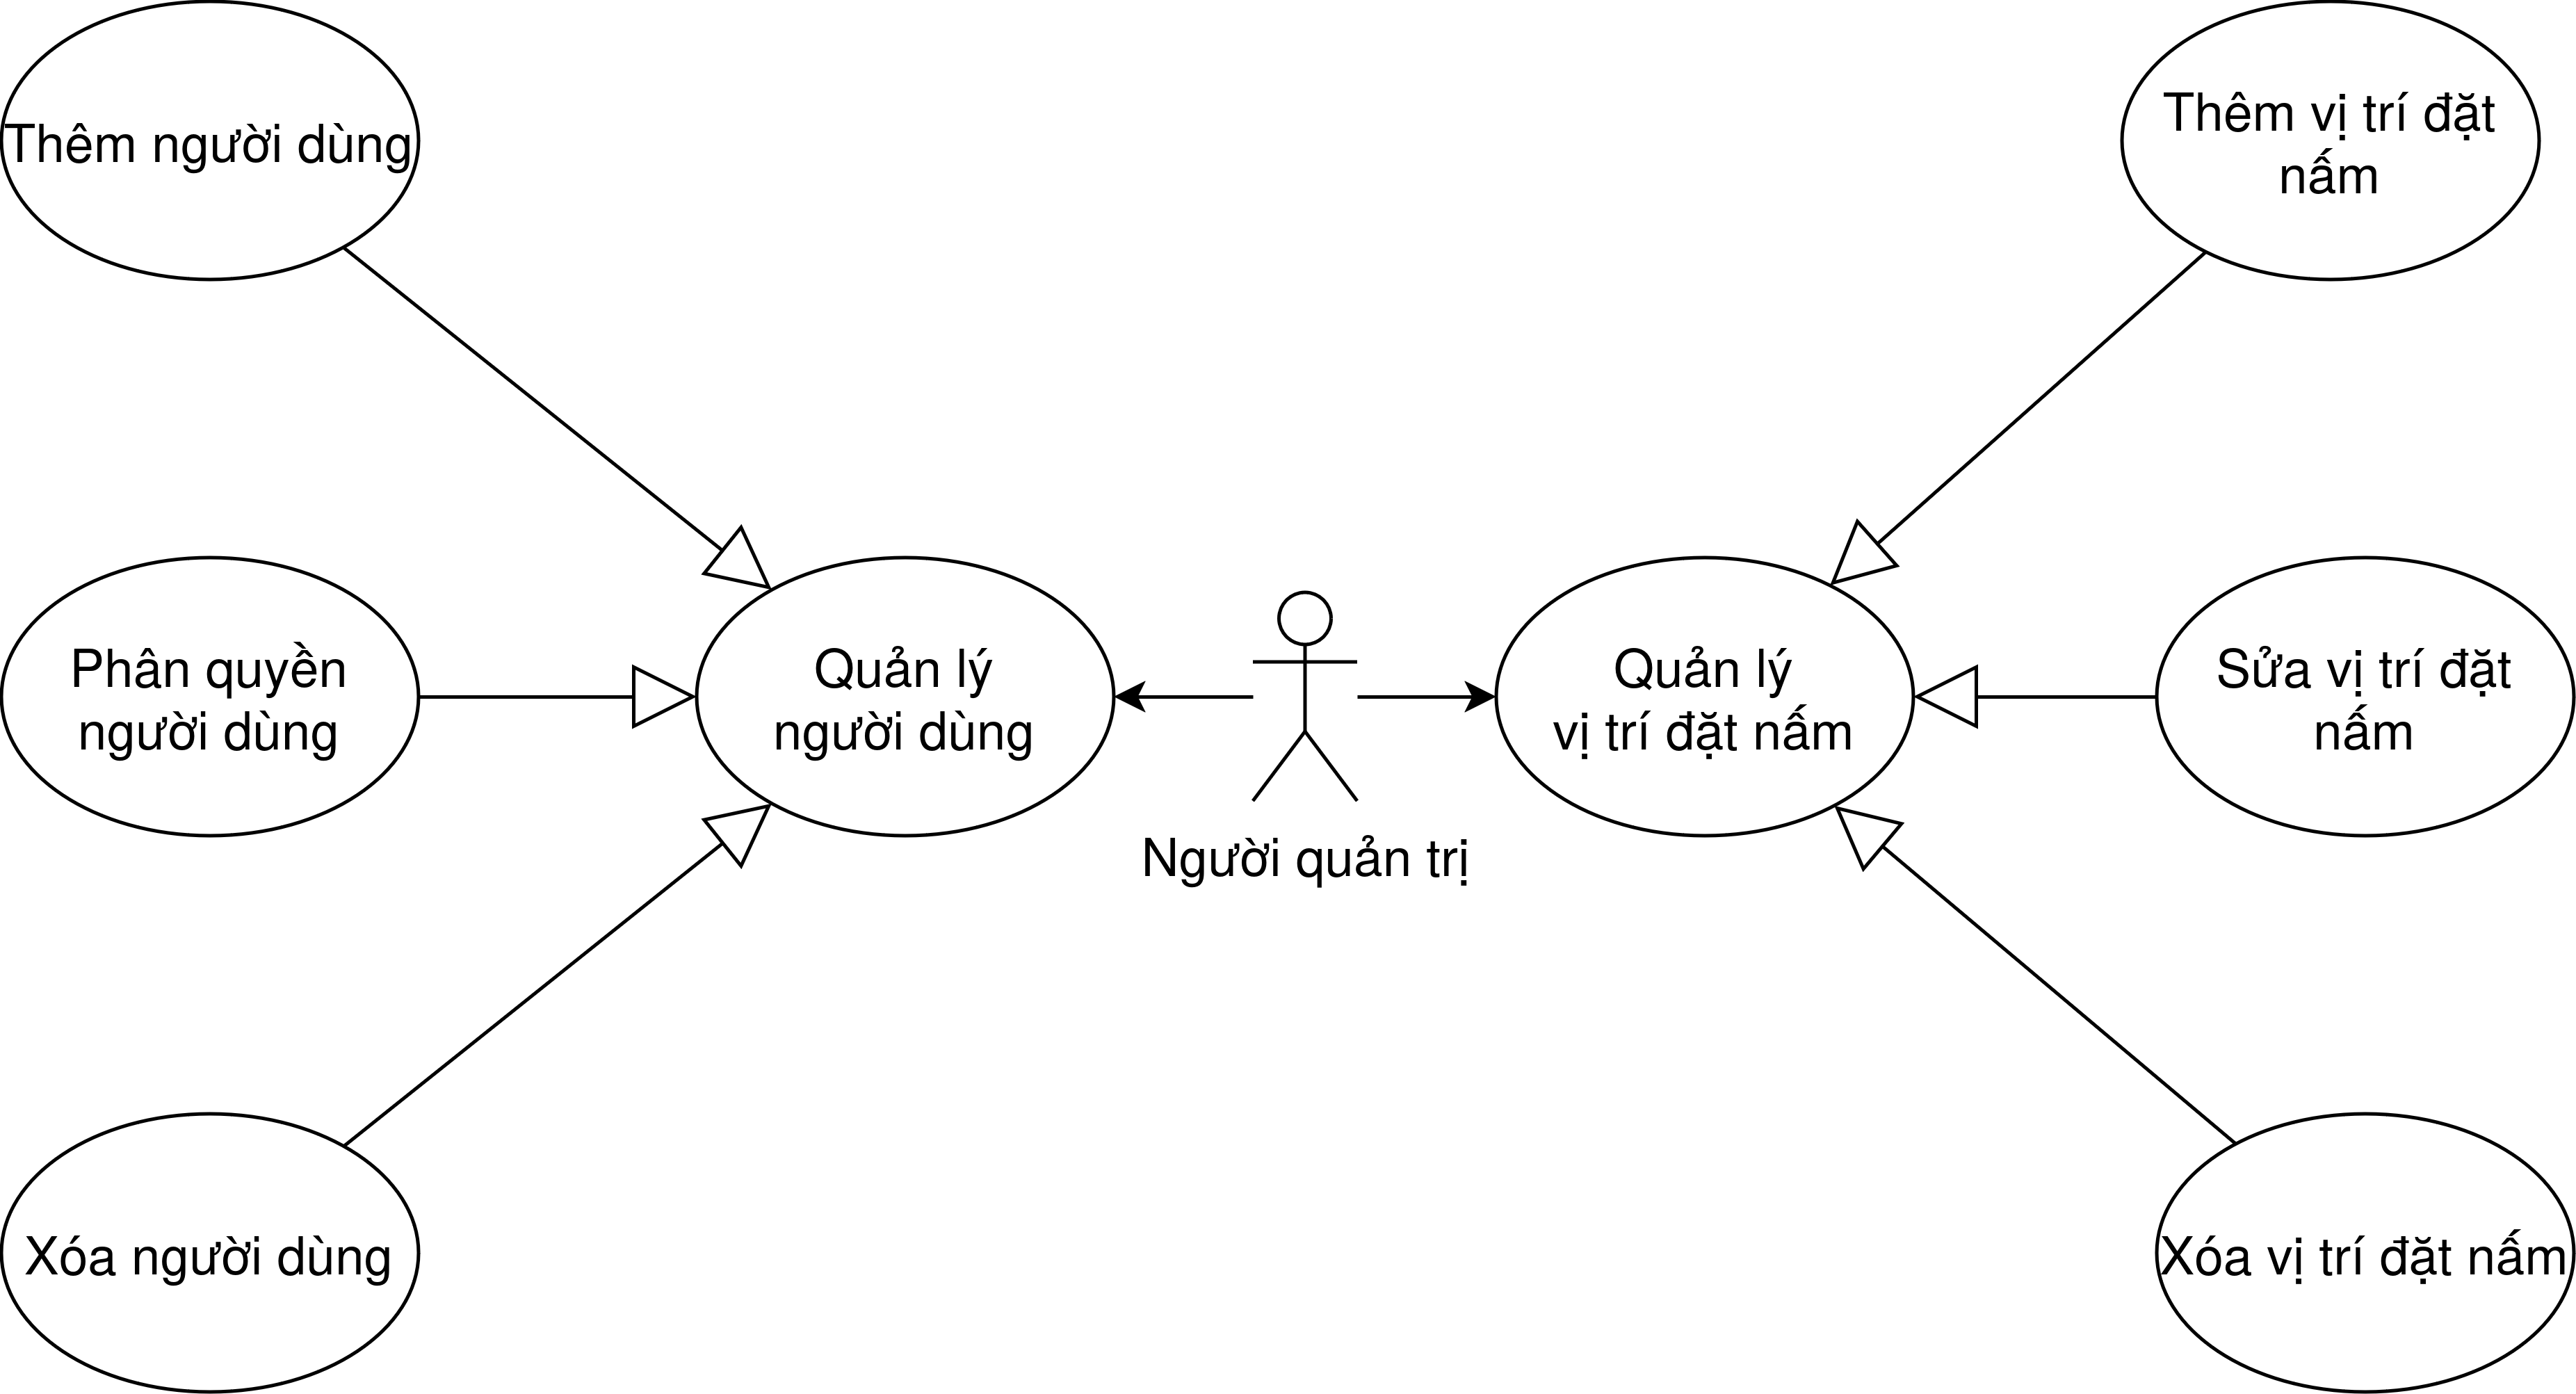
\includegraphics[width=\linewidth]{images/admin-usecase}
	\caption{Usecase cho người quản trị}
	\label{fig:admin-usecase}
\end{figure}
\subsubsection{Đặc tả usecase thêm người dùng}

% Please add the following required packages to your document preamble:
% \usepackage{longtable}
% Note: It may be necessary to compile the document several times to get a multi-page table to line up properly
\begin{longtable}[c]{|l|p{11cm}|}
	\caption{Đặc tả usecase thêm người dùng}
	\label{tab:des-create-user}\\
	\hline
\textbf{Usecase} & \textbf{Nội dung}                                                                                  \\ \hline
\endfirsthead
\hline
\textbf{Usecase}    & \textbf{Nội dung}                                                                                              \\ \hline
\endhead
	%
	Tên usecase      & Thêm người dùng                                                                        \\ \hline
	Mô tả               & Cho phép người quản trị tạo tài khoản người dùng với quyền hạn tương ứng.                                                \\ \hline
	Người dùng          & Người quản trị hệ thống                                                              \\ \hline
	Điều kiện kích hoạt & Người quản trị muốn tạo tài khoản cho người theo dõi hoặc người quản lý chăm sóc nấm hoặc người quản trị khác.\\ \hline
	Tiền điều kiện      & Tên tài khoản không tồn tại                                                          \\ \hline
	Hậu điều kiện       & Tài khoản tạo thành công.                                                             \\ \hline
	Luồng sự kiện chính &
	\begin{tabular}[c]{p{10.5cm}}
		1. Người quản trị nhấn vào mục “User Management”. \\ 
		2. Hệ thống hiển thị trang quản trị người dùng với danh sách người dùng hiện tại.\\
		3. Người quản trị nhập tên người dùng và mật khẩu, chọn quyền hạn và nhấn "Add".\\ 
		4. Hệ thống tải lại trang với danh sách người dùng mới.
	\end{tabular} \\ \hline
	Luồng sự kiện thay thế &
	\begin{tabular}[c]{p{10.5cm}}
		\textbf{- Người dùng đã tồn tại}\\ 
		4. Hệ thống tải lại trang, danh sách người dùng không thay đổi.
	\end{tabular} \\ \hline
	
\end{longtable}
\subsubsection{Đặc tả usecase phân quyền người dùng}

% Please add the following required packages to your document preamble:
% \usepackage{longtable}
% Note: It may be necessary to compile the document several times to get a multi-page table to line up properly
\begin{longtable}[c]{|l|p{11cm}|}
	\caption{Đặc tả usecase phân quyền người dùng}
	\label{tab:des-update-role}\\
	\hline
\textbf{Usecase} & \textbf{Nội dung}                                                                                  \\ \hline
\endfirsthead
\hline
\textbf{Usecase}    & \textbf{Nội dung}                                                                                              \\ \hline
\endhead
	%
	Tên usecase      & Phân quyền người dùng                                                                        \\ \hline
	Mô tả               & Cho phép người quản trị thay đổi quyền hạn cho người dùng.                                      \\ \hline
	Người dùng          & Người quản trị hệ thống                                                              \\ \hline
	Điều kiện kích hoạt & Người quản trị muốn xóa quyền hạn hoặc thay đổi quyền hạn cho người sử dụng.\\ \hline
	Tiền điều kiện      &Người sử dụng tồn tại trong hệ thống.                                                          \\ \hline
	Hậu điều kiện       & Thay đổi quyền hạn thành công.                                                             \\ \hline
	Luồng sự kiện chính &
	\begin{tabular}[c]{p{10.5cm}}
		1. Người quản trị nhấn vào mục “User Management”. \\ 
		2. Hệ thống hiển thị trang quản trị người dùng với danh sách người dùng hiện tại.\\
		3. Người quản trị chọn quyền hạn cho người dùng tương ứng tại cột "Role". \\ 
		4. Hệ thống tải lại trang với danh sách người dùng cùng quyền hạn mới.
	\end{tabular} \\ \hline
	Luồng sự kiện thay thế & Không \\ \hline
	
\end{longtable}

\subsubsection{Đặc tả usecase xóa người dùng}

% Please add the following required packages to your document preamble:
% \usepackage{longtable}
% Note: It may be necessary to compile the document several times to get a multi-page table to line up properly
\begin{longtable}[c]{|l|p{11cm}|}
	\caption{Đặc tả usecase xóa người dùng}
	\label{tab:des-delete-user}\\
	\hline
\textbf{Usecase} & \textbf{Nội dung}                                                                                  \\ \hline
\endfirsthead
\hline
\textbf{Usecase}    & \textbf{Nội dung}                                                                                              \\ \hline
\endhead
	%
	Tên usecase      & Xóa người dùng                                                                        \\ \hline
	Mô tả               & Cho phép người quản trị xóa người dùng.                                      \\ \hline
	Người dùng          & Người quản trị hệ thống                                                              \\ \hline
	Điều kiện kích hoạt & Người quản trị muốn xóa người sử dụng.\\ \hline
	Tiền điều kiện      & Người sử dụng tồn tại trong hệ thống.                                                          \\ \hline
	Hậu điều kiện       & Xóa người dùng hạn thành công.                                                             \\ \hline
	Luồng sự kiện chính &
	\begin{tabular}[c]{p{10.5cm}}
		1. Người quản trị nhấn vào mục “User Management”. \\ 
		2. Hệ thống hiển thị trang quản trị người dùng với danh sách người dùng hiện tại.\\
		3. Người quản trị nhấn "Remove" người dùng muốn xóa. \\ 
		4. Hệ thống tải lại trang với danh sách người dùng mới.
	\end{tabular} \\ \hline
	Luồng sự kiện thay thế & Không \\ \hline
	
\end{longtable}

\subsubsection{Đặc tả usecase thêm vị trí đặt nấm}

% Please add the following required packages to your document preamble:
% \usepackage{longtable}
% Note: It may be necessary to compile the document several times to get a multi-page table to line up properly
\begin{longtable}[c]{|l|p{11cm}|}
	\caption{Đặc tả usecase thêm vị trí đặt nấm}
	\label{tab:des-create-position}\\
	\hline
\textbf{Usecase} & \textbf{Nội dung}                                                                                  \\ \hline
\endfirsthead
\hline
\textbf{Usecase}    & \textbf{Nội dung}                                                                                              \\ \hline
\endhead
	%
	Tên usecase      & Thêm vị trí đặt nấm                                                                        \\ \hline
	Mô tả               & Cho phép người quản trị thêm vị trí đặt nấm vào hệ thống.                                      \\ \hline
	Người dùng          & Người quản trị hệ thống                                                              \\ \hline
	Điều kiện kích hoạt & Người quản trị muốn thêm vị trí đặt nấm.\\ \hline
	Tiền điều kiện      & Tọa độ vị trí đặt nấm không tồn tại.                                                          \\ \hline
	Hậu điều kiện       & Thêm vị trí đặt nấm thành công.                                                             \\ \hline
	Luồng sự kiện chính &
	\begin{tabular}[c]{p{10.5cm}}
		1. Người quản trị nhấn vào mục “Position Management”. \\ 
		2. Hệ thống hiển thị trang quản trị với danh sách các vị trí hiện tại và một dòng thêm vị trí mới.\\
		3. Người quản trị nhập tọa độ vị trí muốn thêm và nhấn "Add". \\ 
		4. Hệ thống tải lại trang với danh sách vị trí mới.
	\end{tabular} \\ \hline
	Luồng sự kiện thay thế & Không \\ \hline
\end{longtable}

\subsubsection{Đặc tả usecase sửa vị trí đặt nấm}

% Please add the following required packages to your document preamble:
% \usepackage{longtable}
% Note: It may be necessary to compile the document several times to get a multi-page table to line up properly
\begin{longtable}[c]{|l|p{11cm}|}
	\caption{Đặc tả usecase sửa vị trí đặt nấm}
	\label{tab:des-update-position}\\
	\hline
\textbf{Usecase} & \textbf{Nội dung}                                                                                  \\ \hline
\endfirsthead
\hline
\textbf{Usecase}    & \textbf{Nội dung}                                                                                              \\ \hline
\endhead
	%
	Tên usecase      & Sửa vị trí đặt nấm                                                                        \\ \hline
	Mô tả               & Cho phép người quản trị sửa tọa độ vị trí đặt nấm trong hệ thống.                                      \\ \hline
	Người dùng          & Người quản trị hệ thống                                                              \\ \hline
	Điều kiện kích hoạt & Người quản trị muốn sửa tọa độ vị trí đặt nấm.\\ \hline
	Tiền điều kiện      & Vị trí đặt nấm tồn tại trong hệ thống.                                                          \\ \hline
	Hậu điều kiện       & Sửa vị trí đặt nấm thành công.                                                             \\ \hline
	Luồng sự kiện chính &
	\begin{tabular}[c]{p{10.5cm}}
		1. Người quản trị nhấn vào mục “Position Management”. \\ 
		2. Hệ thống hiển thị trang quản trị với danh sách các vị trí hiện tại và một dòng thêm vị trí mới.\\
		3. Người quản trị nhập tọa độ vị trí muốn sửa với vị trí tương ứng và nhấn "Update". \\ 
		4. Hệ thống tải lại trang với danh sách vị trí mới.
	\end{tabular} \\ \hline
	Luồng sự kiện thay thế & Không \\ \hline
\end{longtable}

\subsubsection{Đặc tả usecase xóa vị trí đặt nấm}

% Please add the following required packages to your document preamble:
% \usepackage{longtable}
% Note: It may be necessary to compile the document several times to get a multi-page table to line up properly
\begin{longtable}[c]{|l|p{11cm}|}
	\caption{Đặc tả usecase xóa vị trí đặt nấm}
	\label{tab:des-delete-position}\\
	\hline
\textbf{Usecase} & \textbf{Nội dung}                                                                                  \\ \hline
\endfirsthead
\hline
\textbf{Usecase}    & \textbf{Nội dung}                                                                                              \\ \hline
\endhead
	%
	Tên usecase      & Xóa vị trí đặt nấm                                                                        \\ \hline
	Mô tả               & Cho phép người quản trị xóa vị trí đặt nấm trong hệ thống.                                      \\ \hline
	Người dùng          & Người quản trị hệ thống                                                              \\ \hline
	Điều kiện kích hoạt & Người quản trị muốn xóa vị trí đặt nấm.\\ \hline
	Tiền điều kiện      & Vị trí đặt nấm tồn tại trong hệ thống.                                                          \\ \hline
	Hậu điều kiện       & Xóa vị trí đặt nấm thành công.                                                             \\ \hline
	Luồng sự kiện chính &
	\begin{tabular}[c]{p{10.5cm}}
		1. Người quản trị nhấn vào mục “Position Management”. \\ 
		2. Hệ thống hiển thị trang quản trị với danh sách các vị trí hiện tại và một dòng thêm vị trí mới.\\
		3. Người quản trị nhấn "Delete" tại vị trí muốn xóa tương ứng.\\ 
		4. Hệ thống tải lại trang với danh sách vị trí mới.
	\end{tabular} \\ \hline
	Luồng sự kiện thay thế & Không \\ \hline
\end{longtable}

\section{Thiết kế hệ thống theo dõi và chăm sóc nấm}

\subsection{Sơ đồ đối tượng}
Trong hệ thống theo dõi và chăm sóc nấm, các thành phần phải liên hệ chặt chẽ với nhau. Vì vậy, việc thiết kế thành một khối thống nhất với các mô đun nhỏ sẽ giúp tối ưu hoạt động của hệ thống. Các dối tượng, mô đun trong hệ thống được thể hiện trong hình \ref{fig:diagram-objects}.

\begin{figure}[h]
	\centering
	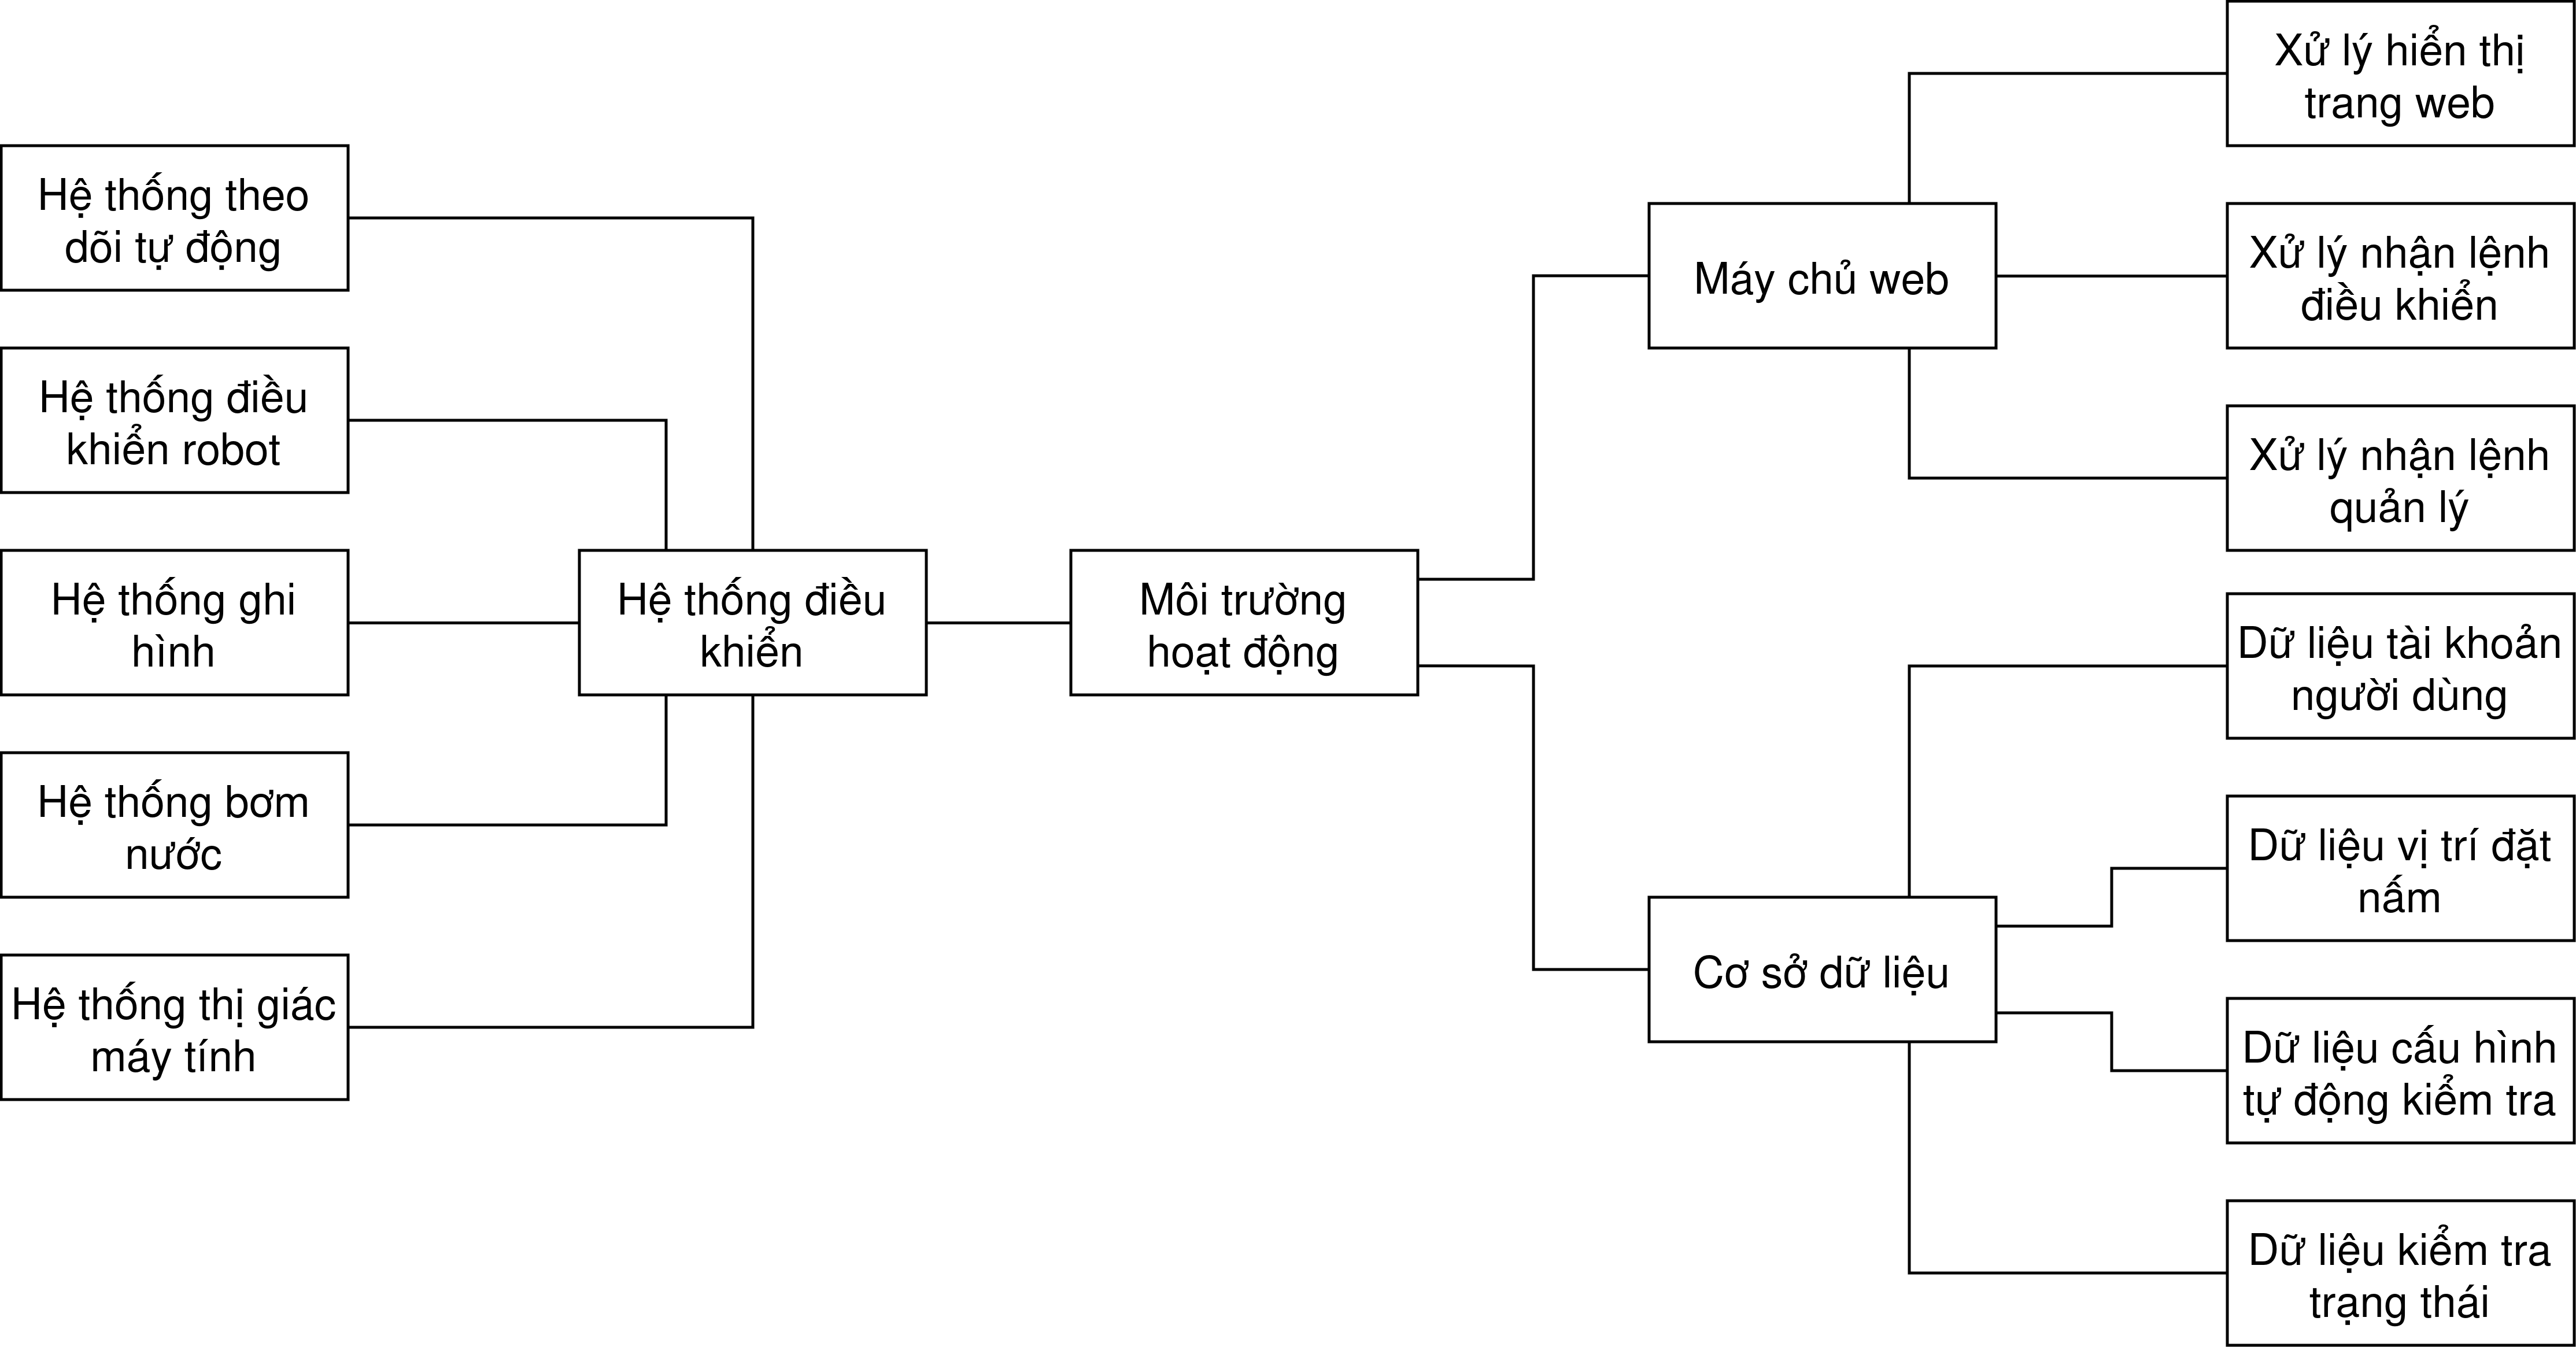
\includegraphics[width=1\linewidth]{images/diagram-objects}
	\caption{Sơ đồ đối tượng trong hệ thống}
	\label{fig:diagram-objects}
\end{figure}

\subsection{Sơ đồ phần cứng}

\begin{figure}[h]
	\centering
	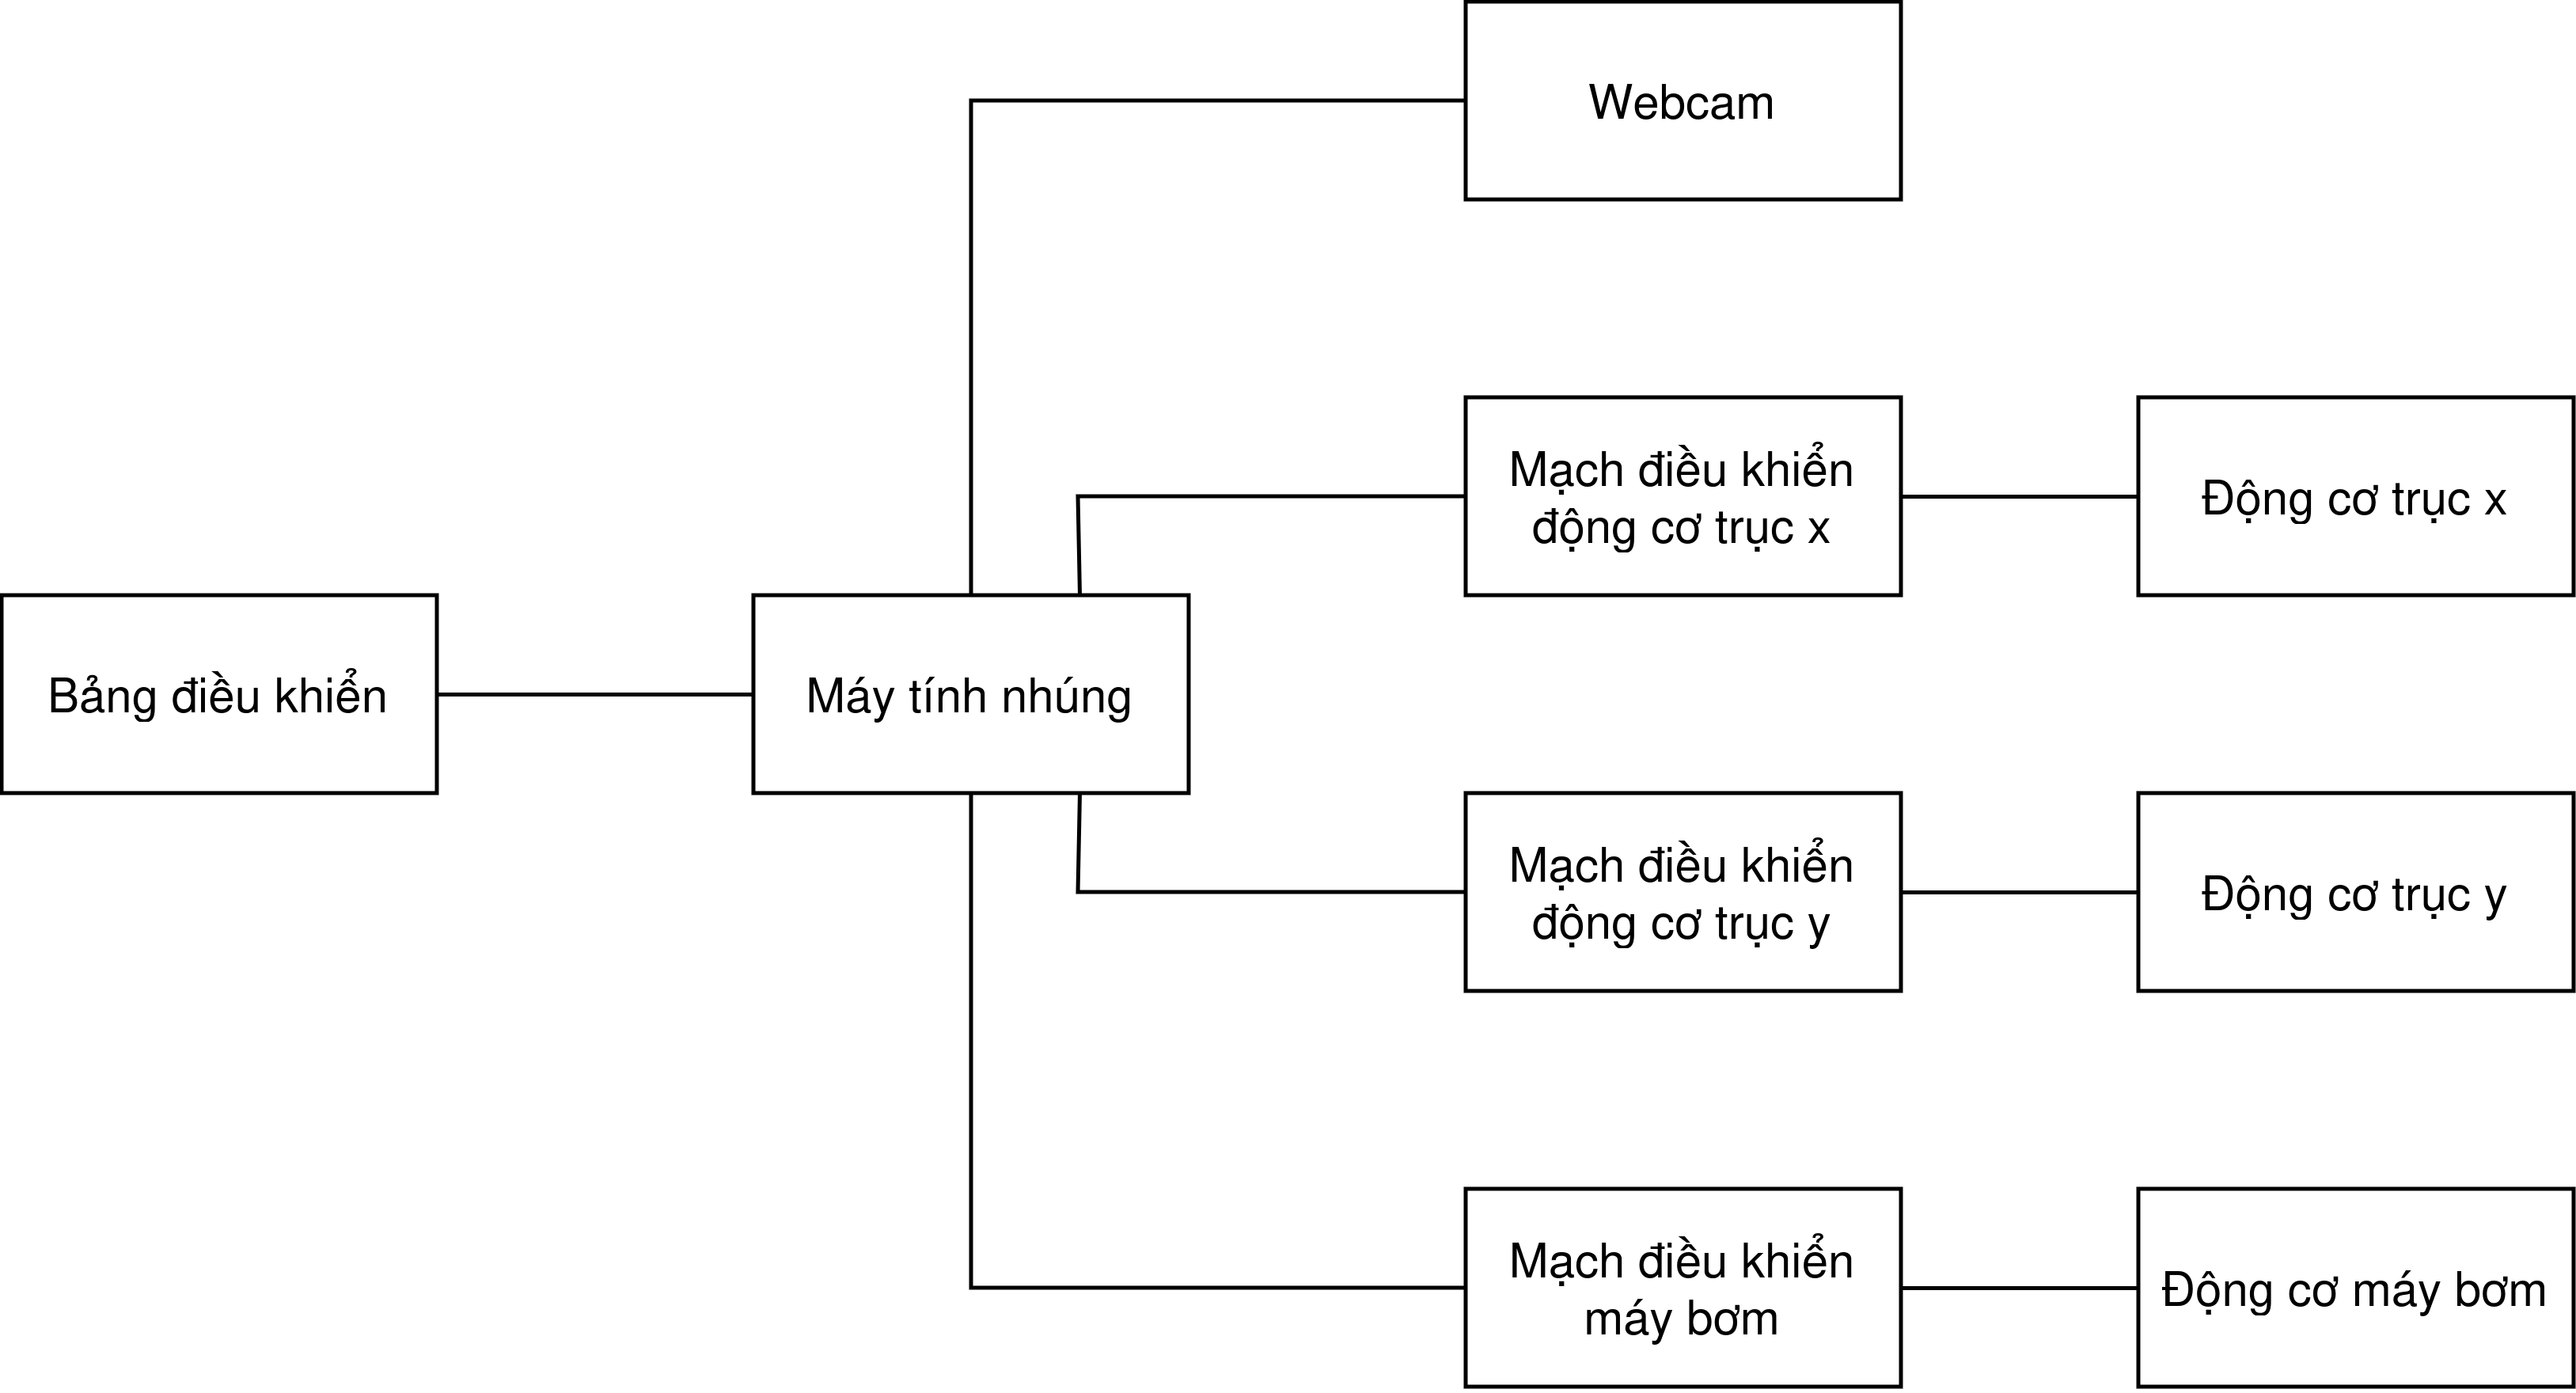
\includegraphics[width=0.7\linewidth]{images/hardware}
	\caption{Sơ đồ phần cứng}
	\label{fig:hardware}
\end{figure}
Hệ thống sử dụng webcam để ghi lại hình ảnh nấm, máy bơm để tưới nước cung cấp độ ẩm cho nấm. Các thiết bị này được di chuyển tới từng vị trí đặt nấm thông qua hai động cơ bước.

Trung tâm của hệ thống là máy tính nhúng giúp điều khiển toàn bộ hoạt động của hệ thống và là nơi lưu trữ dữ liệu. Bảng điều khiển cung cấp giao diện cho người dùng tương tác với hệ thống.





\subsection{Sơ đồ hợp tác}
\subsubsection{Sơ đồ yêu cầu hiển thị trang web}

Các yêu cầu theo dõi hệ thống, truy cập các trang quản lý được gọi chung là yêu cầu hiển thị, được mô tả trong biểu đồ hình \ref{fig:collab-show}.
\begin{figure}[h]
	\centering
	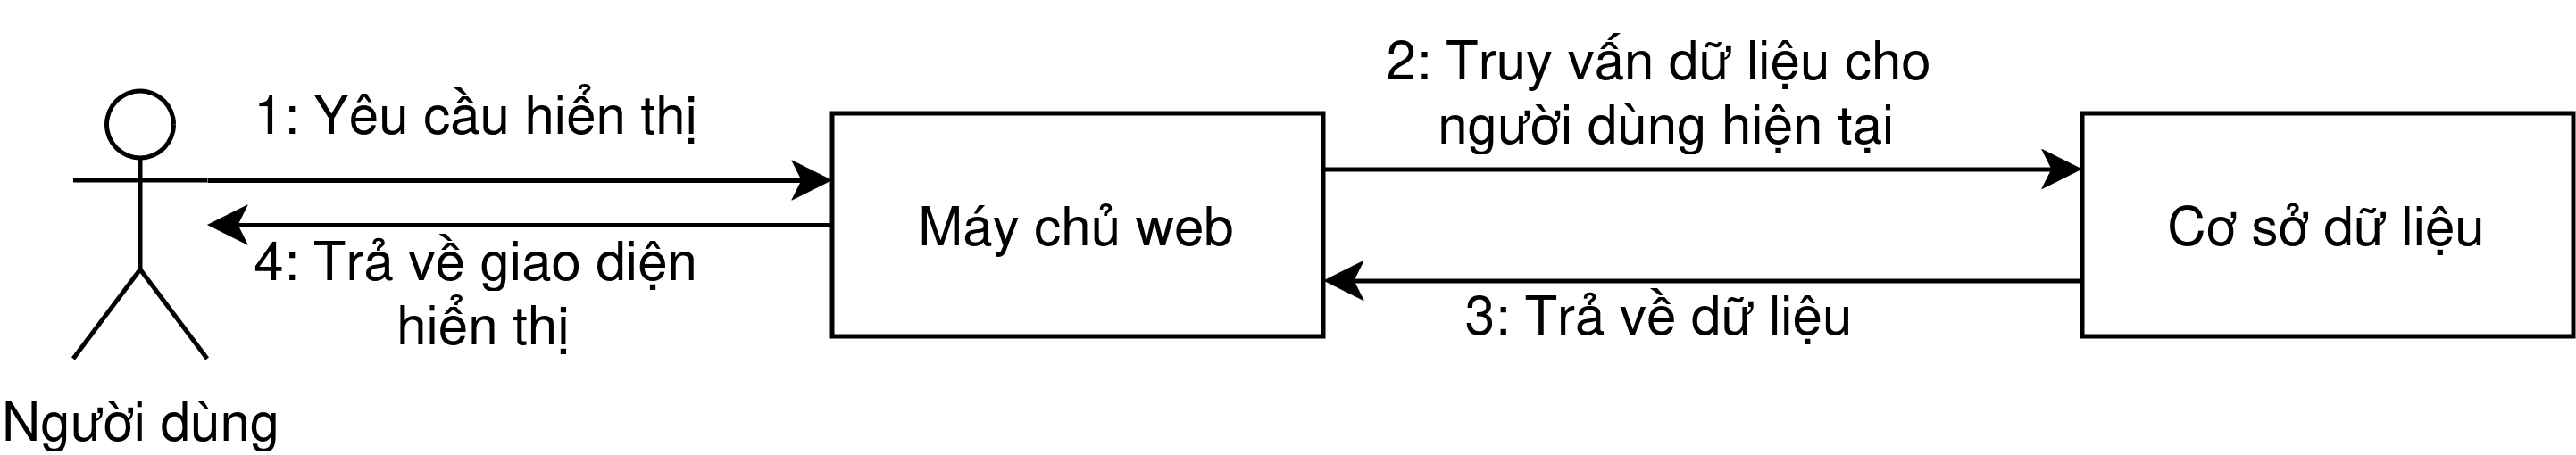
\includegraphics[width=0.8\linewidth]{images/collab-show}
	\caption{Sơ đồ yêu cầu hiển thị trang web}
	\label{fig:collab-show}
\end{figure}

\subsubsection{Sơ đồ yêu cầu cập nhật dữ liệu}
Các yêu cầu cập nhật, xóa bỏ trong quản lý người dùng, quản lý vị trí được gọi chung là yêu cầu cập nhật dữ liệu được mô tả trong hình \ref{fig:collab-update}.
\begin{figure}[H]
	\centering
	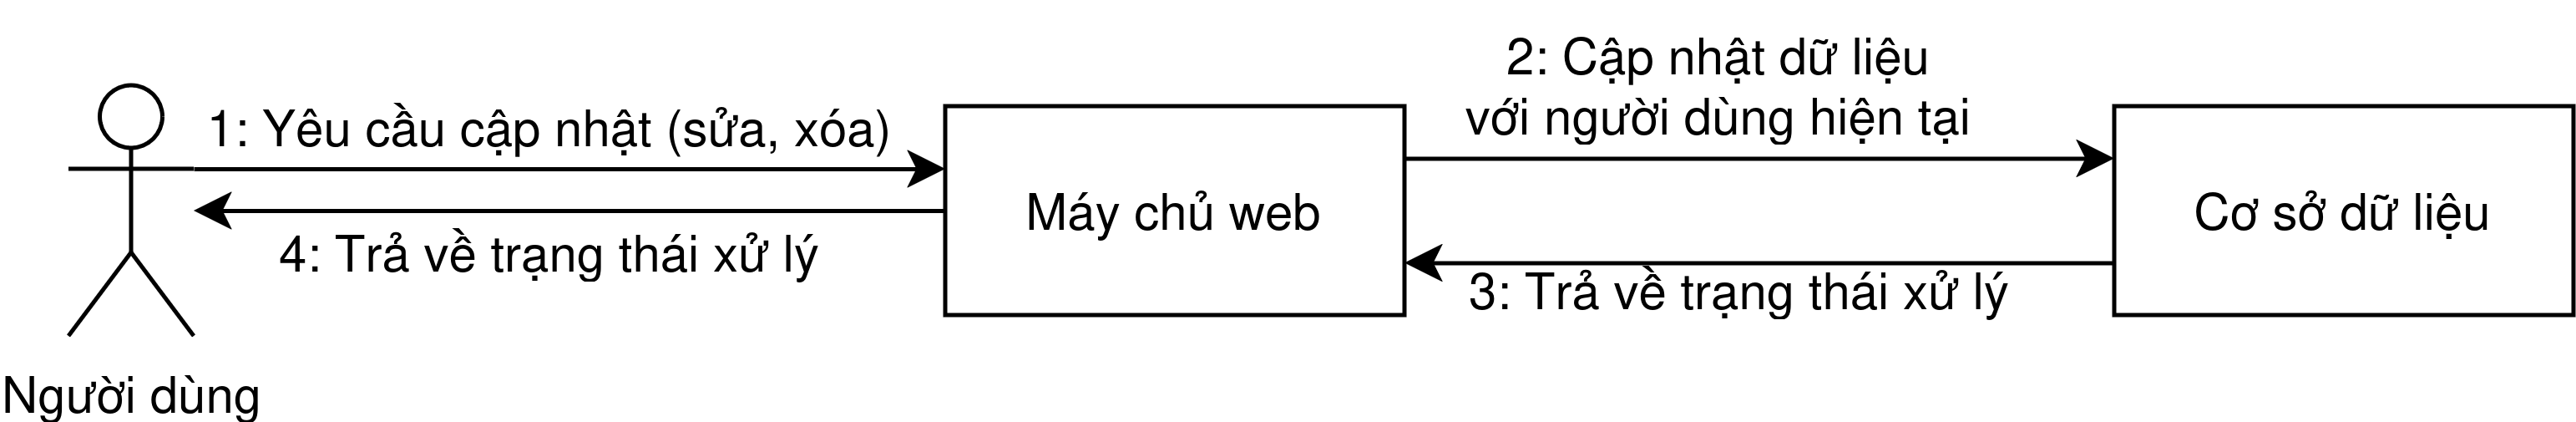
\includegraphics[width=0.8\linewidth]{images/collab-update}
	\caption{Sơ đồ yêu cầu cập nhật dữ liệu}
	\label{fig:collab-update}
\end{figure}

\subsubsection{Sơ đồ yêu cầu điều khiển}
Các yêu cầu kiểm tra, tưới nước từ người dùng được gọi chung là yêu cầu điều khiển, được mô tả trong hình \ref{fig:collab-control}.
\begin{figure}[h]
	\centering
	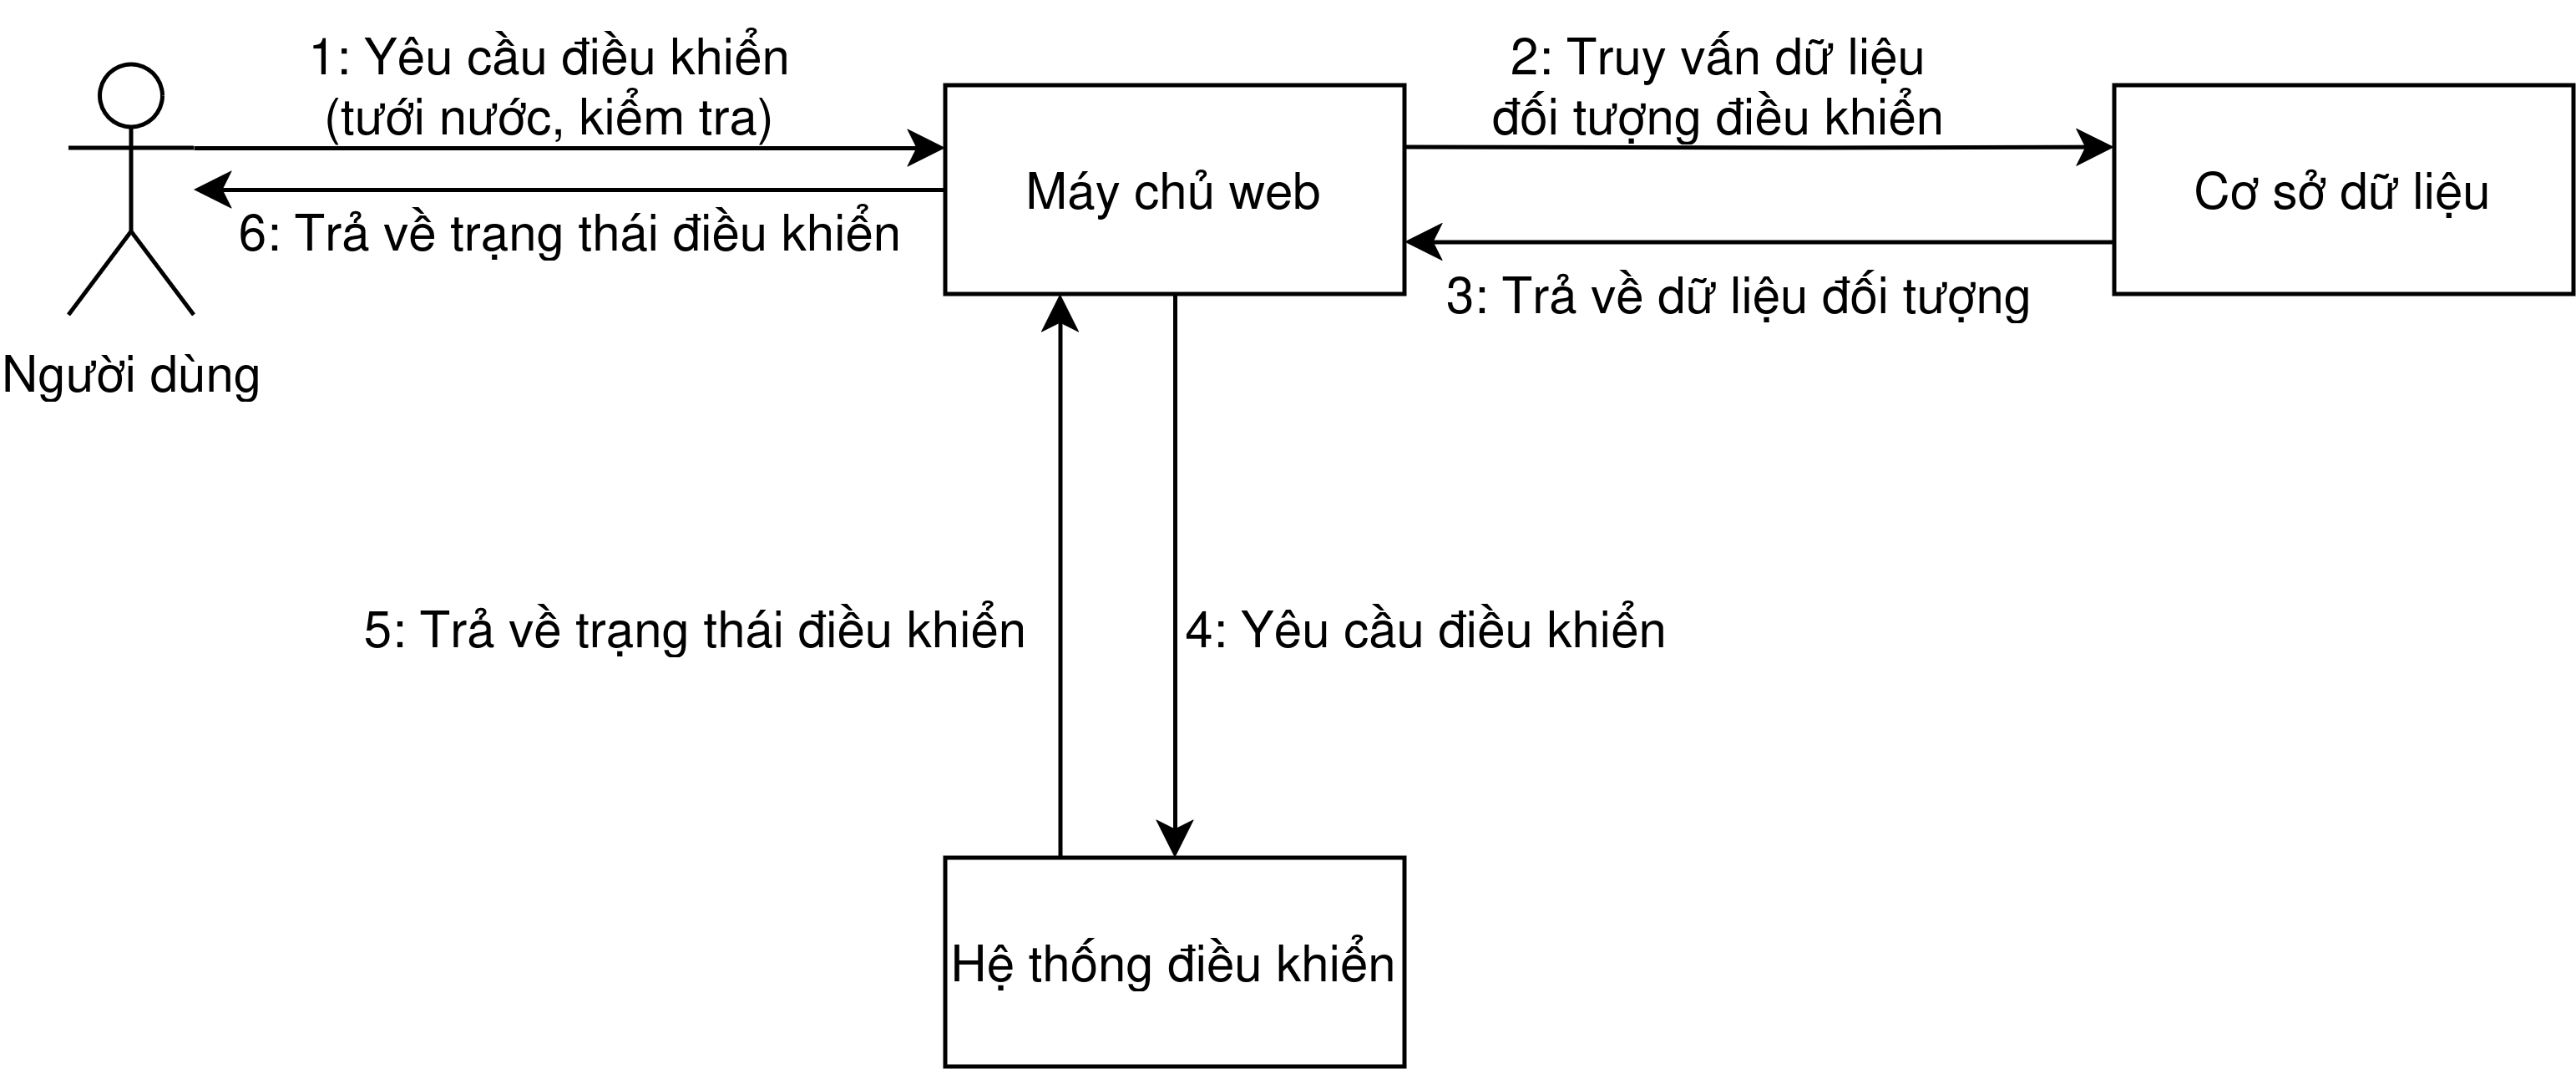
\includegraphics[width=0.8\linewidth]{images/collab-control}
	\caption{Sơ đồ yêu cầu điều khiển}
	\label{fig:collab-control}
\end{figure}

\subsubsection{Sơ đồ theo dõi tự động}
Hoạt động của hệ thống theo dõi tự động được mô tả trong hình \ref{fig:collab-automation}.
\begin{figure}[h]
	\centering
	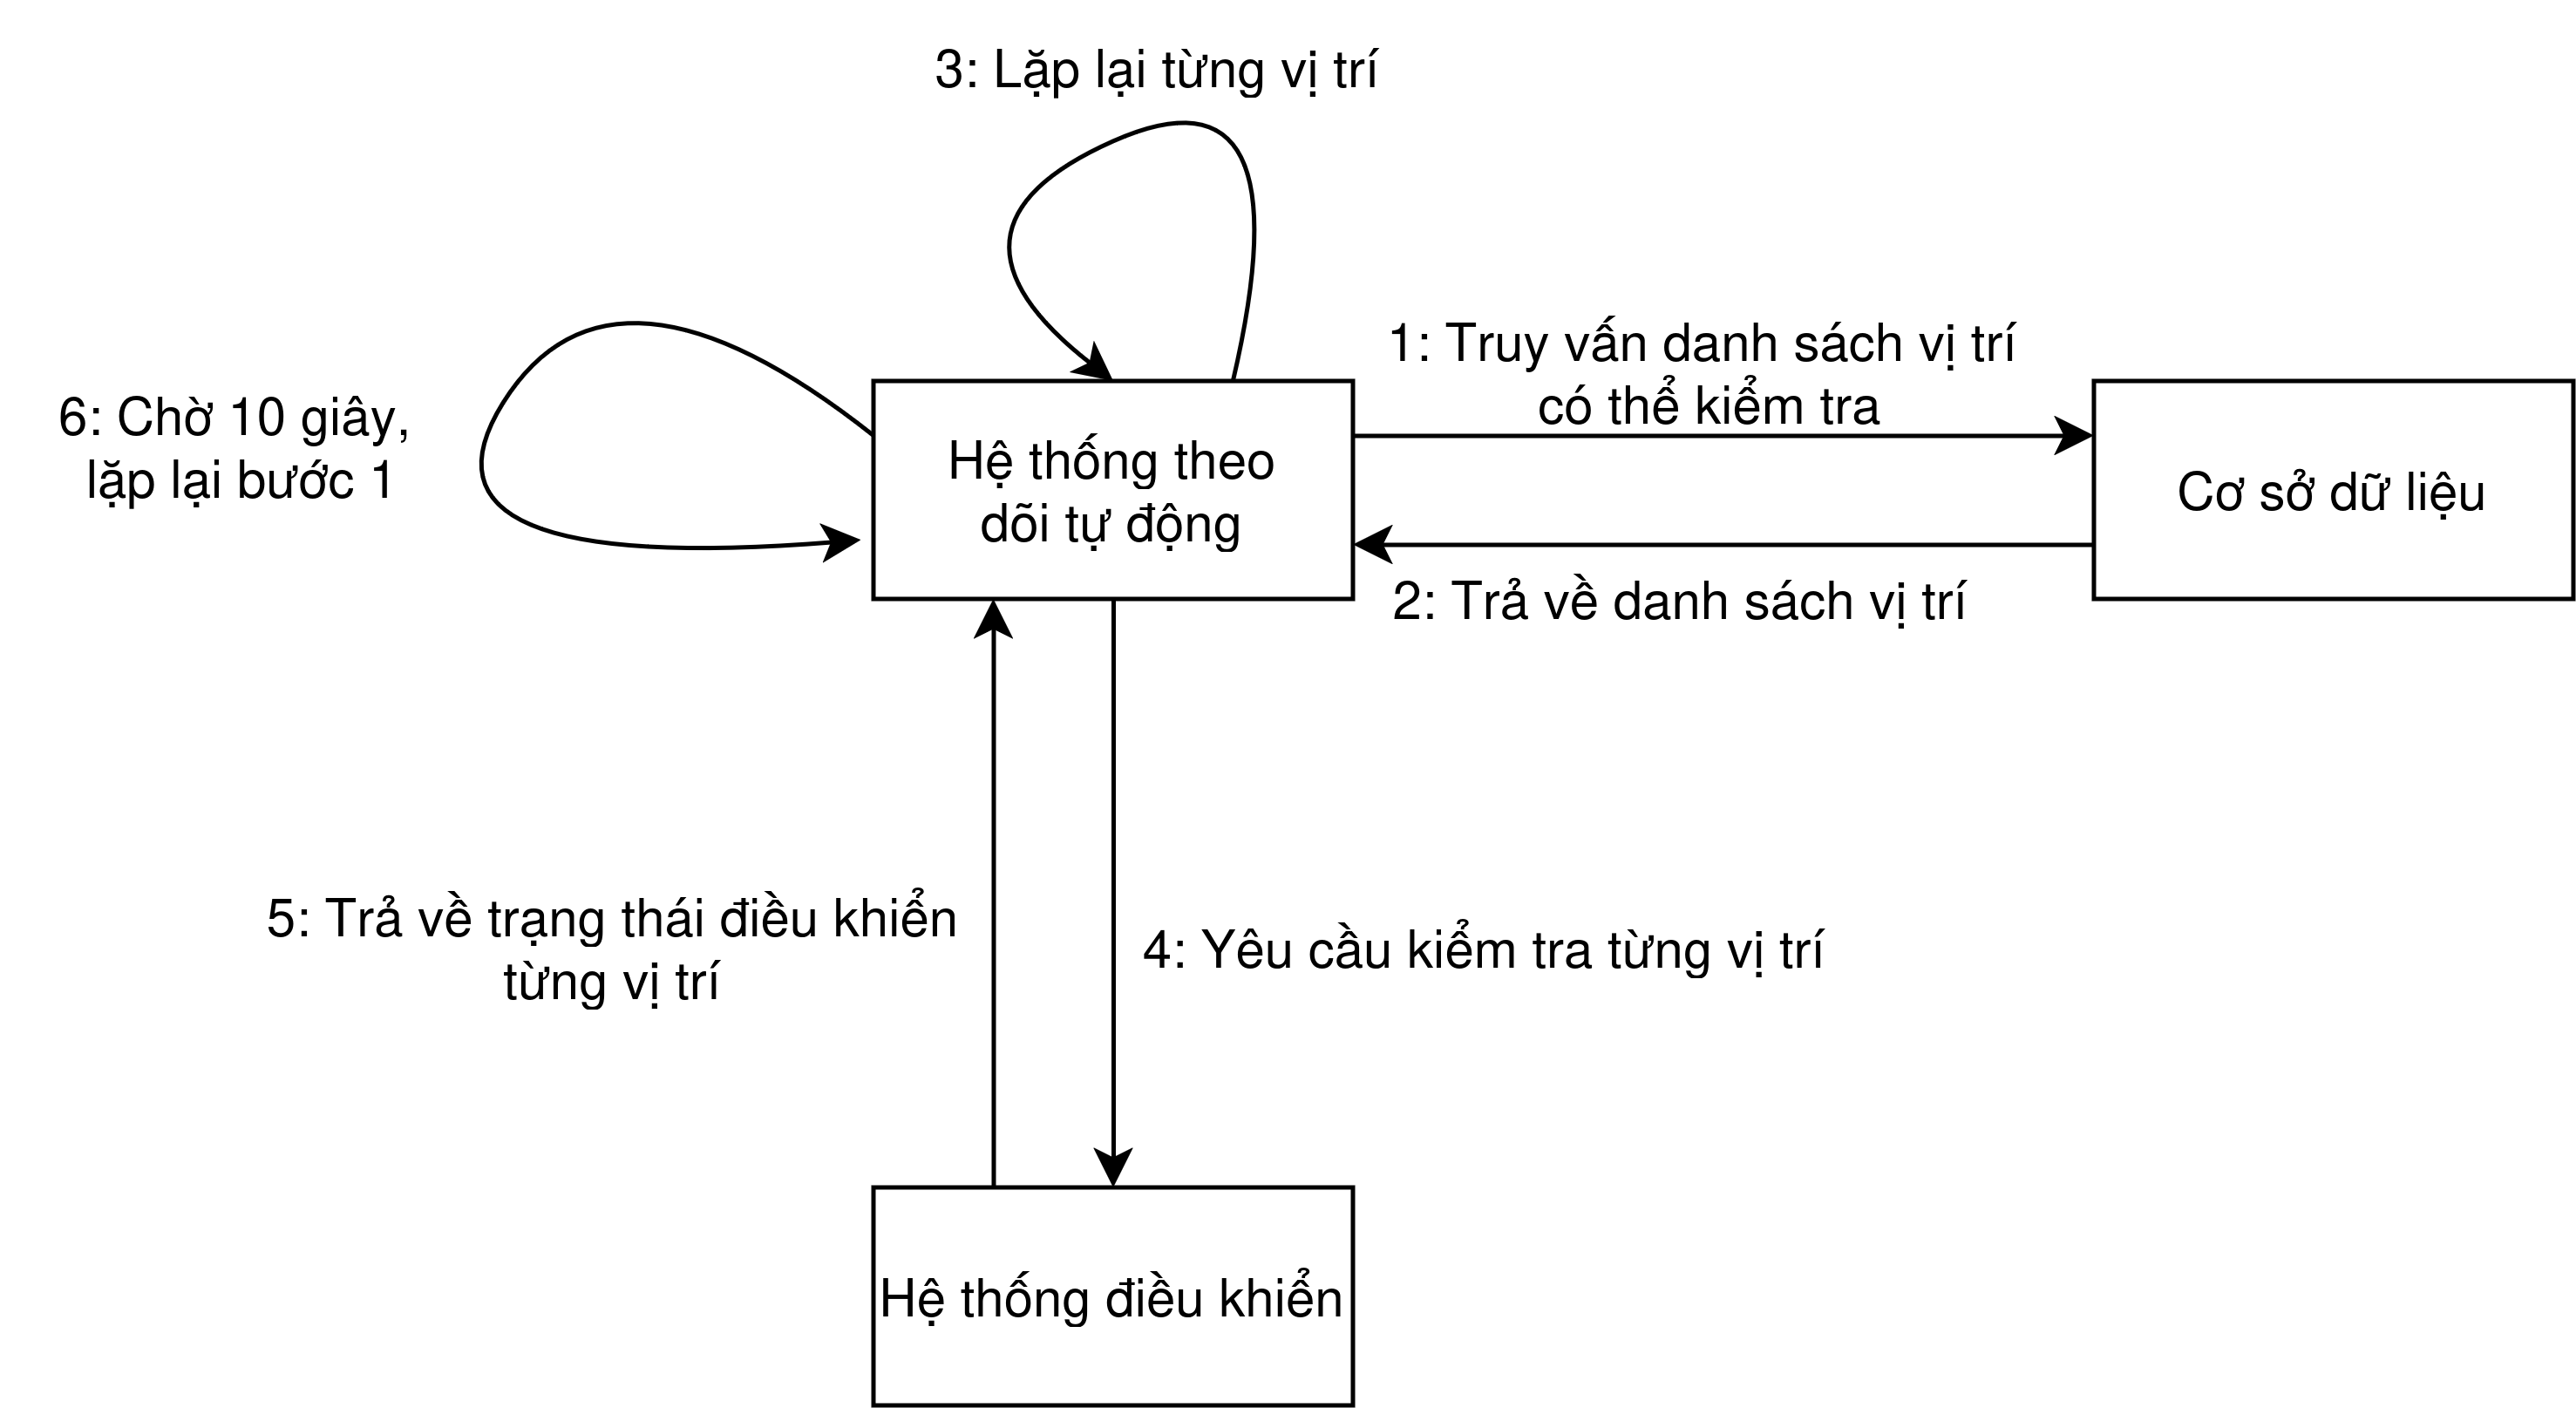
\includegraphics[width=0.8\linewidth]{images/collab-automation}
	\caption{Sơ đồ theo dõi tự động}
	\label{fig:collab-automation}
\end{figure}

\subsubsection{Sơ đồ điều khiển chi tiết}

\begin{figure}[H]
	\centering
	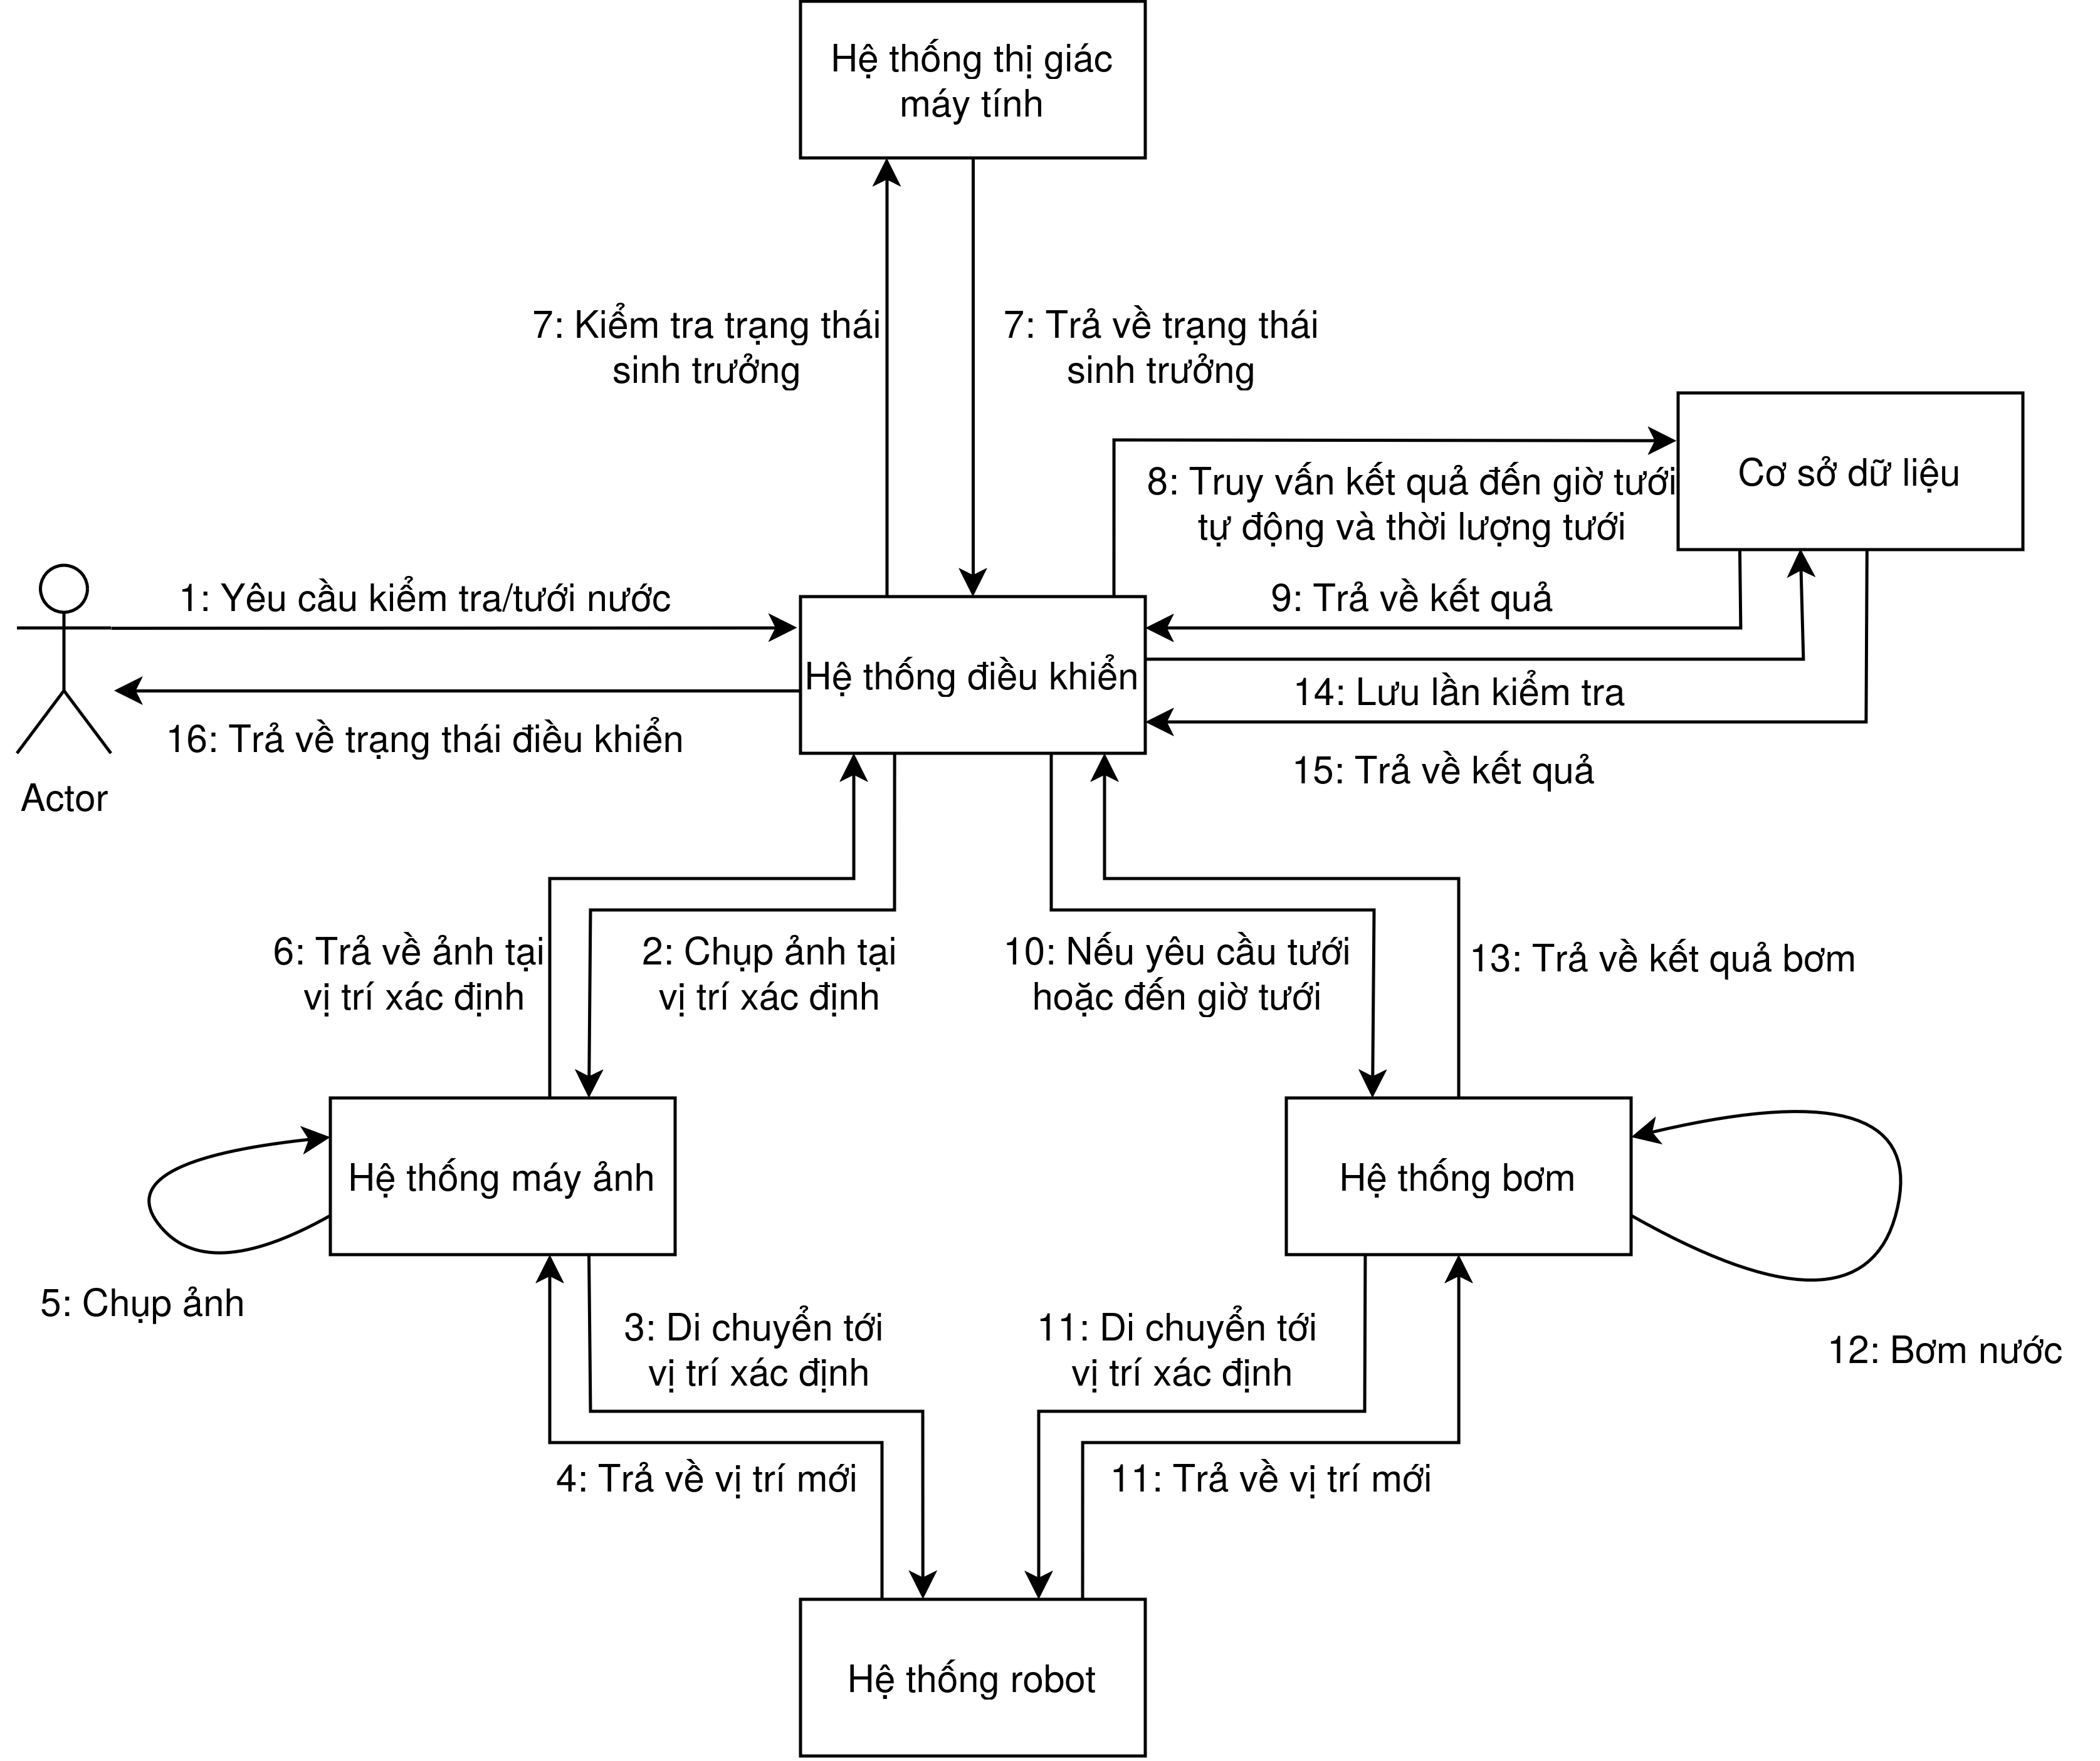
\includegraphics[width=0.8\linewidth]{images/collab-control-detail}
	\caption{Sơ đồ yêu cầu điều khiển chi tiết}
	\label{fig:collab-control-detail}
\end{figure}

Hoạt động của hệ thống điều khiển được mô tả chi tiết trong hình \ref{fig:collab-control-detail}. Tại đây, hệ thống điều khiển gửi lệnh tới hệ thống máy ảnh và hệ thống bơm, hai hệ thống này thực hiện di chuyển tới vị trí tương ứng thông qua hệ thống robot. Dữ liệu hình ảnh được xử lý thông qua hệ thống thị giác máy tính và được xử lý, lưu lại trong cơ sở dữ liệu nhờ hệ thống điều khiển.



\section{Xây dựng tập dữ liệu và huấn luyện mô hình}

\subsection{Thu thập dữ liệu}

Nấm sò trắng là loại nấm phổ biến, được sử dụng nhiều trong các bữa ăn với khả năng chống chịu tốt với điều kiện thời tiết, cho khả năng thu hoạch nhiều lần sau mỗi một tuần. Với số lượng nấm trồng thử là 20 bịch phôi, sau 2 tháng, số lượng nấm thu được tối đa là 160. Số nấm này được lấy hình ảnh phục vụ quá trình thử nghiệm hệ thống.

Ngoài dữ liệu hình ảnh thu được trong thực tế trồng nấm, nguồn ảnh huấn luyện có thể thu thập từ nguồn mạng xã hội.

Trong quá trình trồng thử nghiệm nấm để lấy dữ liệu hình ảnh, nấm được tưới nước với các mức độ khác nhau và hình ảnh được quay phim lại hằng ngày giúp thu được nguồn dữ liệu hình ảnh đa dạng nhất có thể.

Roboflow là một nền tảng hỗ trợ tốt cho việc chuẩn bị dữ liệu huấn luyện. Dữ liệu huấn luyện có thể được tải lên Roboflow dưới dạng ảnh hoặc dạng video sau đó chuyển thành từng khung hình.


\subsection{Chuẩn bị dữ liệu huấn luyện}

Sau khi chuẩn bị dữ liệu huấn luyện, thực hiện gán nhãn cho từng vật thể sử dụng nền tảng Roboflow như trong hình \ref{fig:labelling-interface}. Một số nguyên tắc cần tuân thủ để xây dựng tập dữ liệu mạnh bao gồm:
\begin{itemize}
	\item Tất cả vật thể xuất hiện trong hình đều cần được gán nhãn. Vì mô hình YOLO phát hiện tất cả vật thể trong ảnh, nếu không được gán nhãn đầy đủ, mô hình có thể hoạt động không đúng trong quá trình huấn luyện.
	/
	\item Gán nhãn đầy đủ diện tích vật thể, hộp bao cần bao trùm toàn bộ vật thể và hộp bao không được rộng hơn vật thể quá nhiều để tăng tính chính xác cho mô hình.
	
	\item Các vật thể che lấp nhau cũng cần được gán nhãn đầy đủ. Các mô hình phát hiện vật thể nói chung và mô hình YOLO nói riêng sử dụng các mẫu kích thước và hình dạng hộp bao trong quá trình huấn luyện. Vì vậy, khi gán nhãn cho ảnh, những vật thể che lấp nhau nên được gán nhãn cùng các hộp bao như khi chúng không che lấp.
\end{itemize}

\begin{figure}[H]
	\centering
	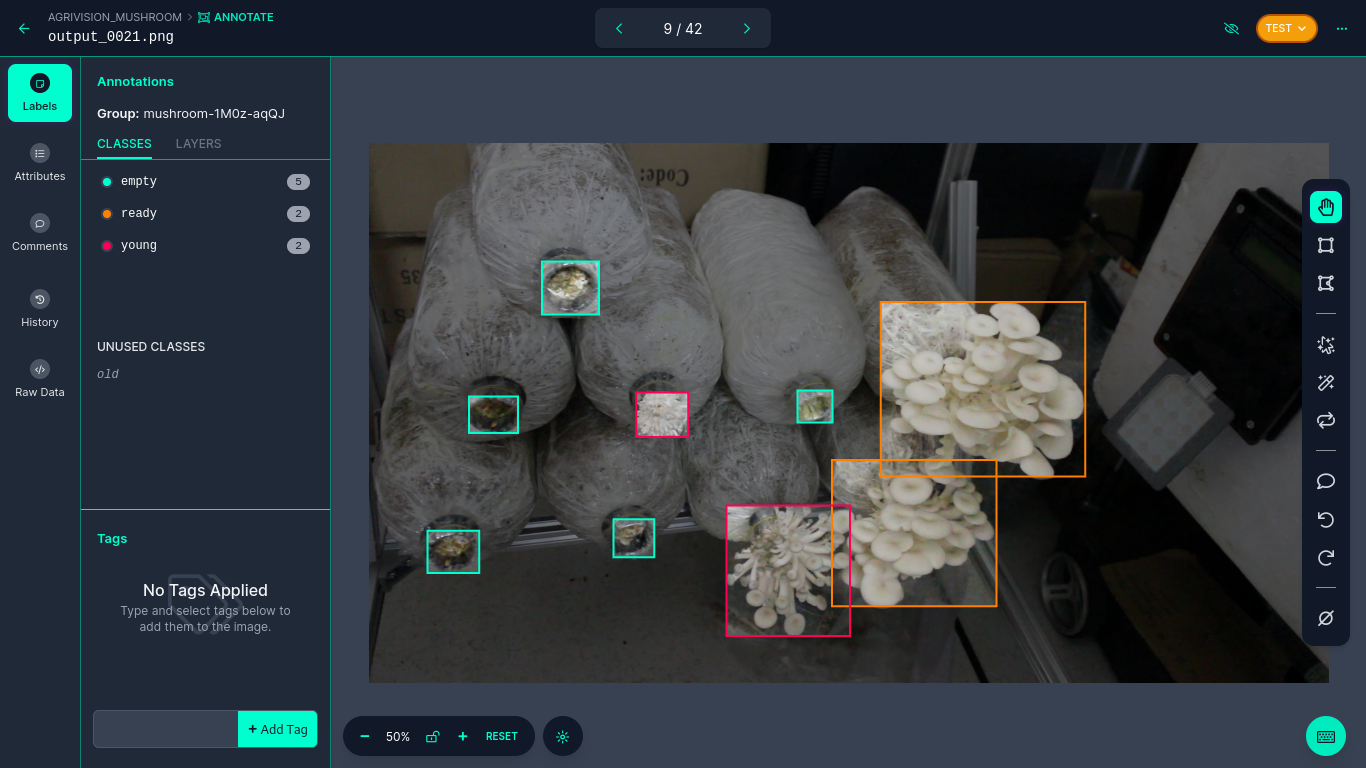
\includegraphics[width=0.7\linewidth]{images/labelling-interface}
	\caption{Giao diện gán nhãn cho nấm}
	\label{fig:labelling-interface}
\end{figure}

\subsection{Gán nhãn ảnh nấm}

Để hệ thống có thể hoạt động với nhiều loại nấm khác nhau, nhãn cho từng giai đoạn phát triển nên được gắn với tên loại nấm. Trong giới hạn của đồ án sử dụng nấm sò trắng, các nhãn chỉ mô tả giai đoạn phát triển của nấm trong các hình \ref{fig:empty}, \ref{fig:young}, \ref{fig:ready}, \ref{fig:old}.

\begin{figure}[h]
	\centering
	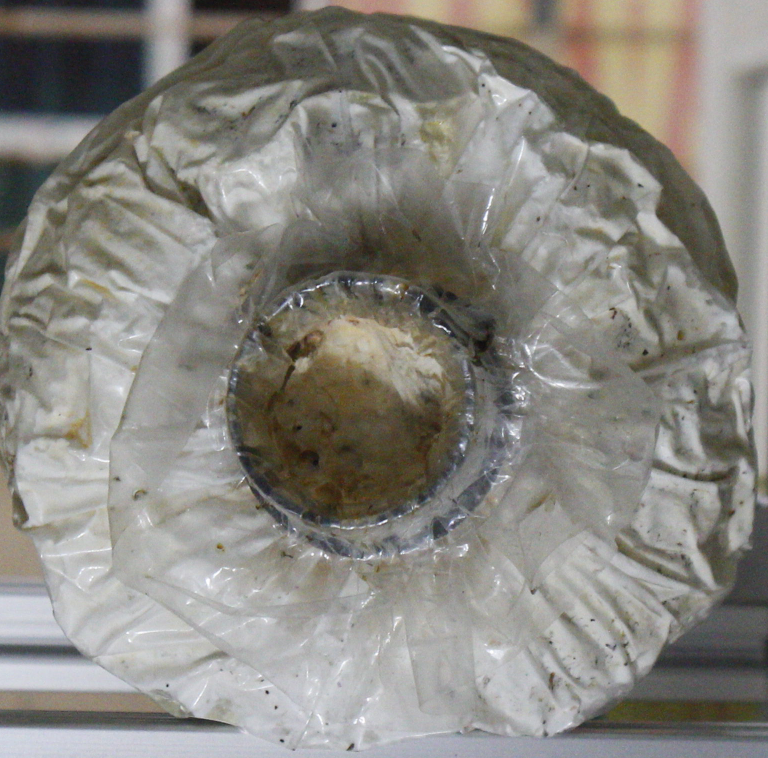
\includegraphics[width=0.4\linewidth]{images/empty}
	\caption{Hình ảnh phôi không có nấm}
	\label{fig:empty}
\end{figure}


Nấm non có thân mọc thẳng về các phía, kích thước tai nấm không lớn hơn thân đáng kể với hình dạng mầu trong hình \ref{fig:young}.

\begin{figure}[H]
    \centering
        \begin{subfigure}{.5\textwidth}
        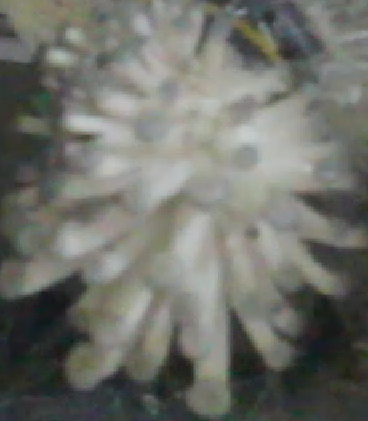
\includegraphics[width=0.8\linewidth]{images/young2.png}
    \end{subfigure}%
    \begin{subfigure}{.5\textwidth}
        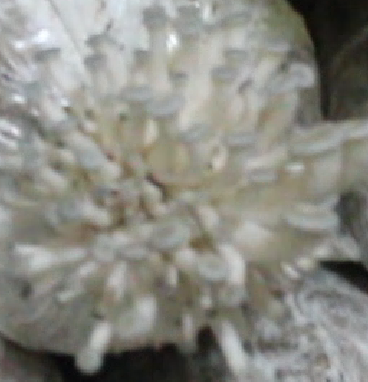
\includegraphics[width=0.8\linewidth]{images/young3.png}
    \end{subfigure}
    \caption{Hình ảnh nấm non}
    \label{fig:young}
\end{figure}

Nấm trưởng thành có tai nấm phát triển, thân nấm uốn cong lên phía trên mô tả trong hình \ref{fig:ready}.

\begin{figure}[H]
    \centering
        \begin{subfigure}{.5\textwidth}
        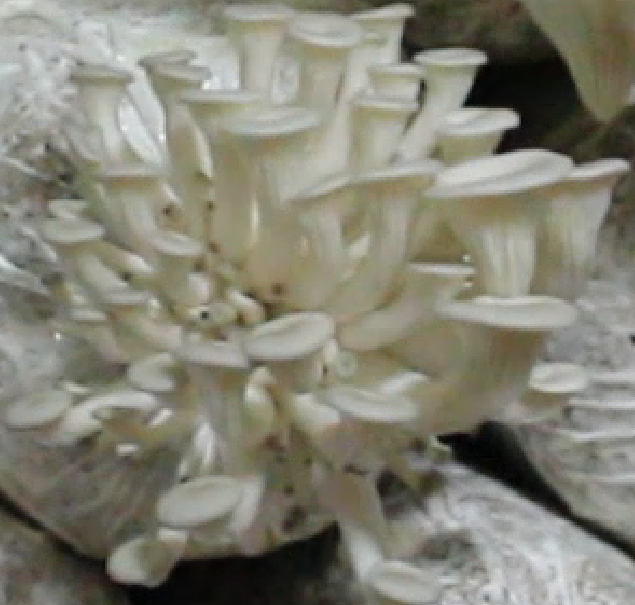
\includegraphics[width=0.8\linewidth]{images/ready1.png}
    \end{subfigure}%
    \begin{subfigure}{.5\textwidth}
        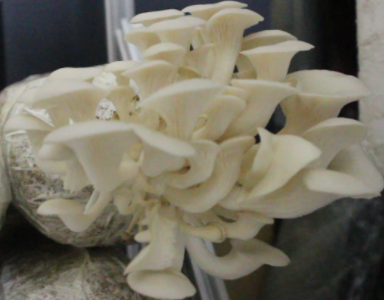
\includegraphics[width=0.8\linewidth]{images/ready3.png}
    \end{subfigure}
    \caption{Hình ảnh nấm trưởng thành, có thể thu hoạch}
    \label{fig:ready}
\end{figure}

Nấm già tai nấm phát triển to có thể bị xoăn lại và chuyển sang màu vàng., thân nấm nhỏ như hình \ref{fig:old}.
\begin{figure}[H]
    \centering
    \begin{subfigure}{.5\textwidth}
        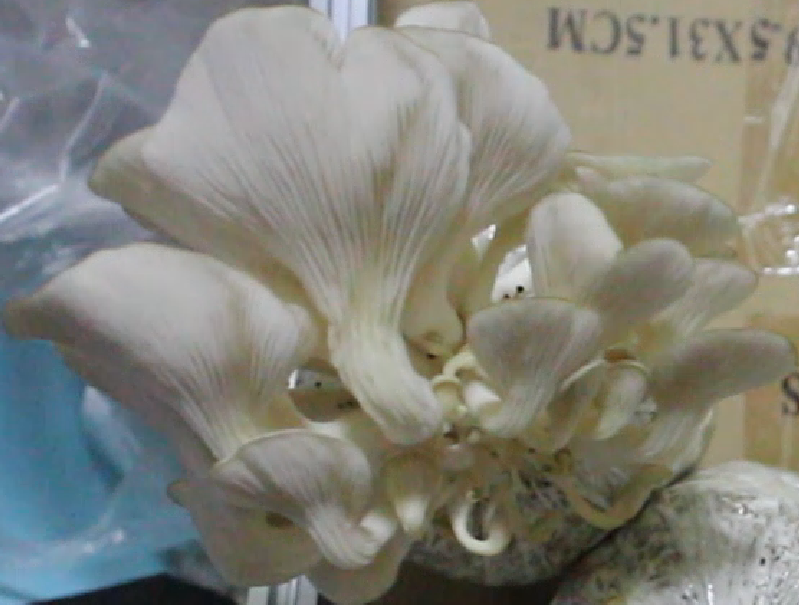
\includegraphics[width=0.85\linewidth]{images/old1.png}
    \end{subfigure}%
    \begin{subfigure}{.5\textwidth}
        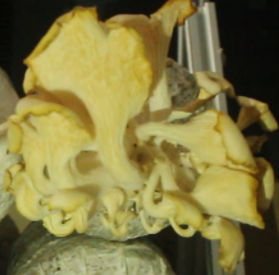
\includegraphics[width=0.85\linewidth]{images/old3.png}
    \end{subfigure}
    \caption{Hình ảnh nấm già}
    \label{fig:old}
\end{figure}

Tổng số hình ảnh được gán nhãn là 852, trong mỗi ảnh có thể có nhiều nấm, trong đó tổng số nấm non là 1135, số nấm trưởng thành là 1274, số nấm già là 526 và số phôi trống là 1622\cite{agrivision_mushroom_dataset}. Số lượng cụ thể cho các tập huấn luyện, tập xác nhận cho mỗi vòng huấn luyện và tập kiểm tra để đánh giá kết quả huấn luyện được thể hiện trong hình \ref{fig:dataset}.

\begin{figure}[H]
	\centering
	\begin{subfigure}{0.8\textwidth}
		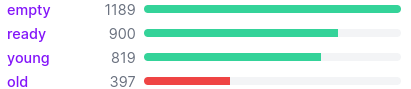
\includegraphics{images/dataset-train}
		\caption{Tập huấn luyện}
	\end{subfigure}
	\begin{subfigure}{0.8\textwidth}
		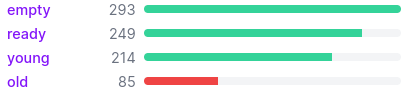
\includegraphics{images/dataset-val}
		\caption{Tập xác nhận}
	\end{subfigure}
	\begin{subfigure}{0.8\textwidth}
		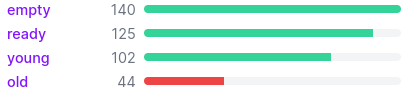
\includegraphics{images/dataset-test}
		\caption{Tập kiểm tra}
	\end{subfigure}
	\caption{Số lượng lớp trong tập dữ liệu}
	\label{fig:dataset}
\end{figure}

Dữ liệu hình ảnh sau khi được gán nhãn cần được xử lý và làm giàu trước khi huấn luyện. Đầu tiên ảnh cần được thay đổi kích thước về kích thước phù hợp với mô hình. Đối với YOLOv8, tỉ lệ kích thước không ảnh hưởng tới kết quả huấn luyện, tuy nhiên, kích thước ảnh huấn luyện cần phù hợp với ảnh sử dụng trong quá trình suy luận. Để phù hợp với ảnh trong quá trình suy luận ảnh sẽ được thay đổi về kích thước 1280x720. Hình ảnh trong tập dữ liệu cũng được làm giàu bằng cách tạo nhiễu.

Sau khi làm giàu, số lượng ảnh được sinh ra là 2086 ảnh. Tập dữ liệu huấn luyện sau khi chuẩn bị đầy đủ sẽ được được tải về và đưa vào huấn luyện. Roboflow hỗ trợ nhiều định dạng khác nhau cho các mạng khác nhau, trong đó có hỗ trợ xuất định dạng tập dữ liệu cho \acrshort{yolo}v8 như hình \ref{fig:export-dataset}.

\begin{figure}[H]
    \centering
    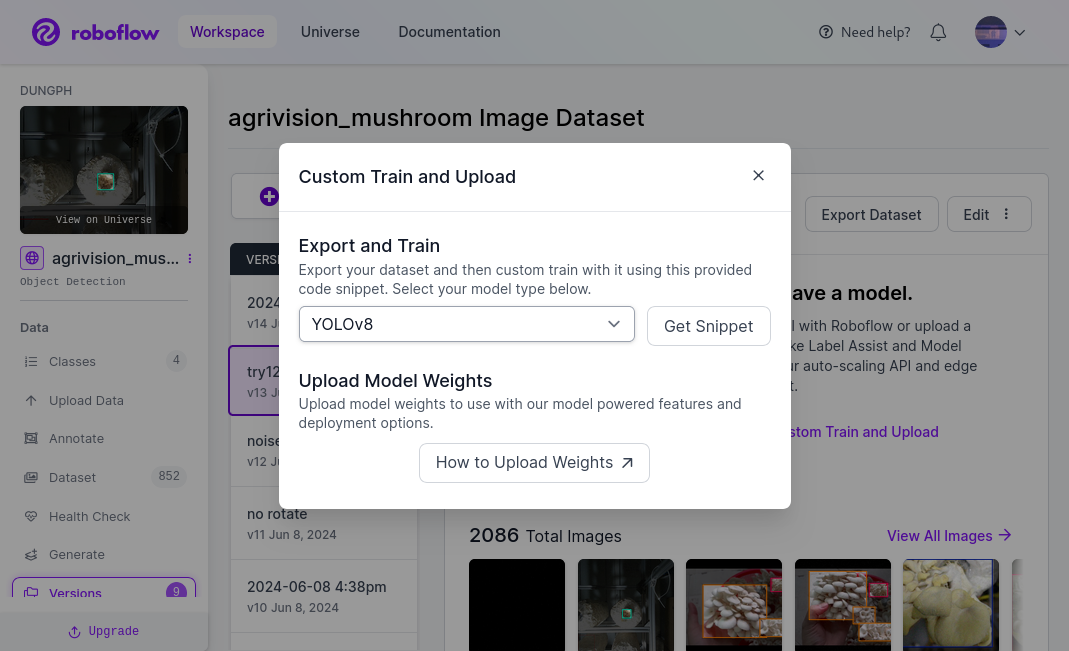
\includegraphics[width=0.85\linewidth]{images/export-dataset.png}
    \caption{Xuất tập dữ liệu huấn luyện}
    \label{fig:export-dataset}
\end{figure}

\subsection{Huấn luyện và đánh giá hiệu suất mô hình}

Ultralytics \cite{yolov8_ultralytics} cung cấp bộ phần mềm hỗ trợ các tác vụ huấn luyện và suy luận sử dụng mô hình \acrshort{yolo} trên các nền tảng hệ điều hành và trên các môi trường trực tuyến như Kaggle. Sử dụng nền tảng Kaggle, do hỗ trợ phần cứng tối ưu, quá trình huấn luyện có thể thực hiện trong thời gian ngắn.

\begin{figure}[h]
	\centering
	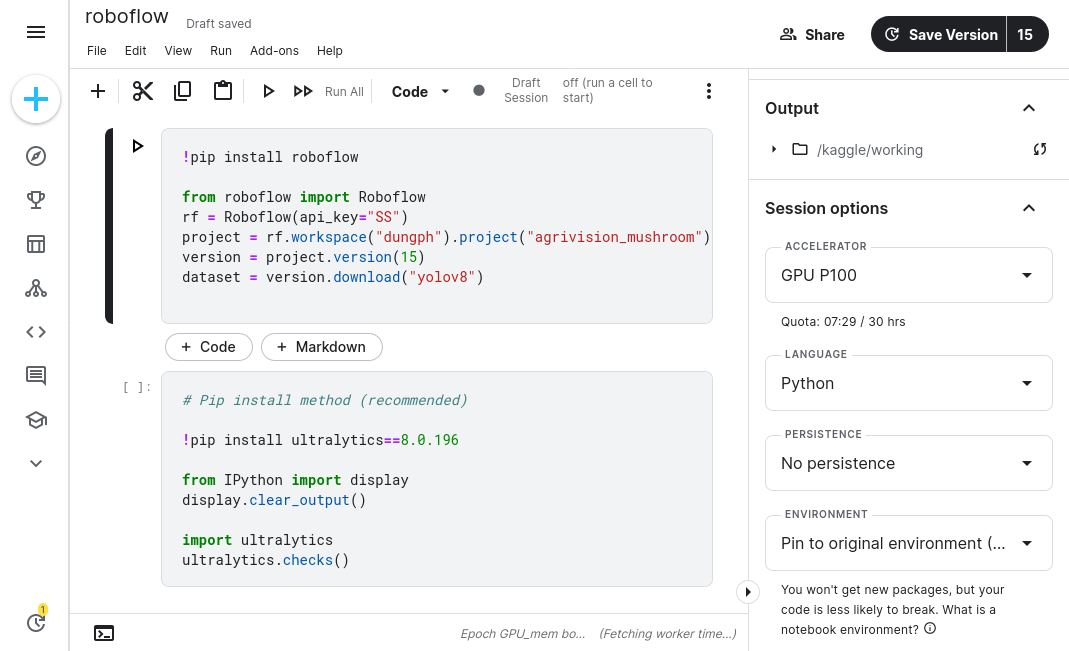
\includegraphics[width=0.9\linewidth]{images/ui-kaggle}
	\caption{Giao diện Kaggle}
	\label{fig:ui-kaggle}
\end{figure}

Các tham số huấn luyện mô hình bao gồm:
\begin{itemize}
	\item Kích thước mô hình YOLO: do số lượng dữ liệu huấn luyện còn nhỏ, mô hình YOLOv8n được sử dụng. Tại đây, chương trình thực hiện tải mô hình đã được huấn luyện từ trước thay vì sử dụng các tham số ngẫu nhiên làm tăng độ phức tạp huấn luyện.
	\item Kích thước hình ảnh (kích thước cạnh dài nhất): sử dụng kích thước 1280px.
	\item Số vòng huấn luyện: khi huấn luyện, nếu chương trình nhận thấy các giá trị mất mát không thể giảm một cách đáng kể, chương trình tự động dừng huấn luyện. Vì vậy, đây là giá trị số vòng huấn luyện tối đa. Giá trị hiện tại epoch = 200.
\end{itemize}

Sau 132 vòng huấn luyện, chương trình tự động dừng lại do không có sự cải thiện đáng kể trong vòng 50 vòng gần nhất. Từ hình \ref{fig:training-result-f1}, mô hình đưa ra kết quả chính xác nhất với hệ số tự tin từ 10\% đến 75\%, hệ số tự tin càng cao càng đưa ra kết quả chính xác trên mỗi dự đoán trong hình \ref{fig:training-result-p} và tỉ lệ phát hiện đúng vật thể bắt đầu giảm rõ rệt khi hệ số tự tin lớn hơn 70\% với biểu đồ trong hình \ref{fig:training-result-r}. Vì vậy, khi triển khai, hệ số tự tin có thể đặt giá trị cao để cho các suy đoán chính xác nhưng không được vượt quá 75\%. Ngược lại, khi cần lượng dự đoán đầy đủ nhất, hệ số tự tin có thể giảm xuống nhưng không giảm quá 10\%

\begin{figure}[H]
    \centering
    \begin{subfigure}{.5\textwidth}
        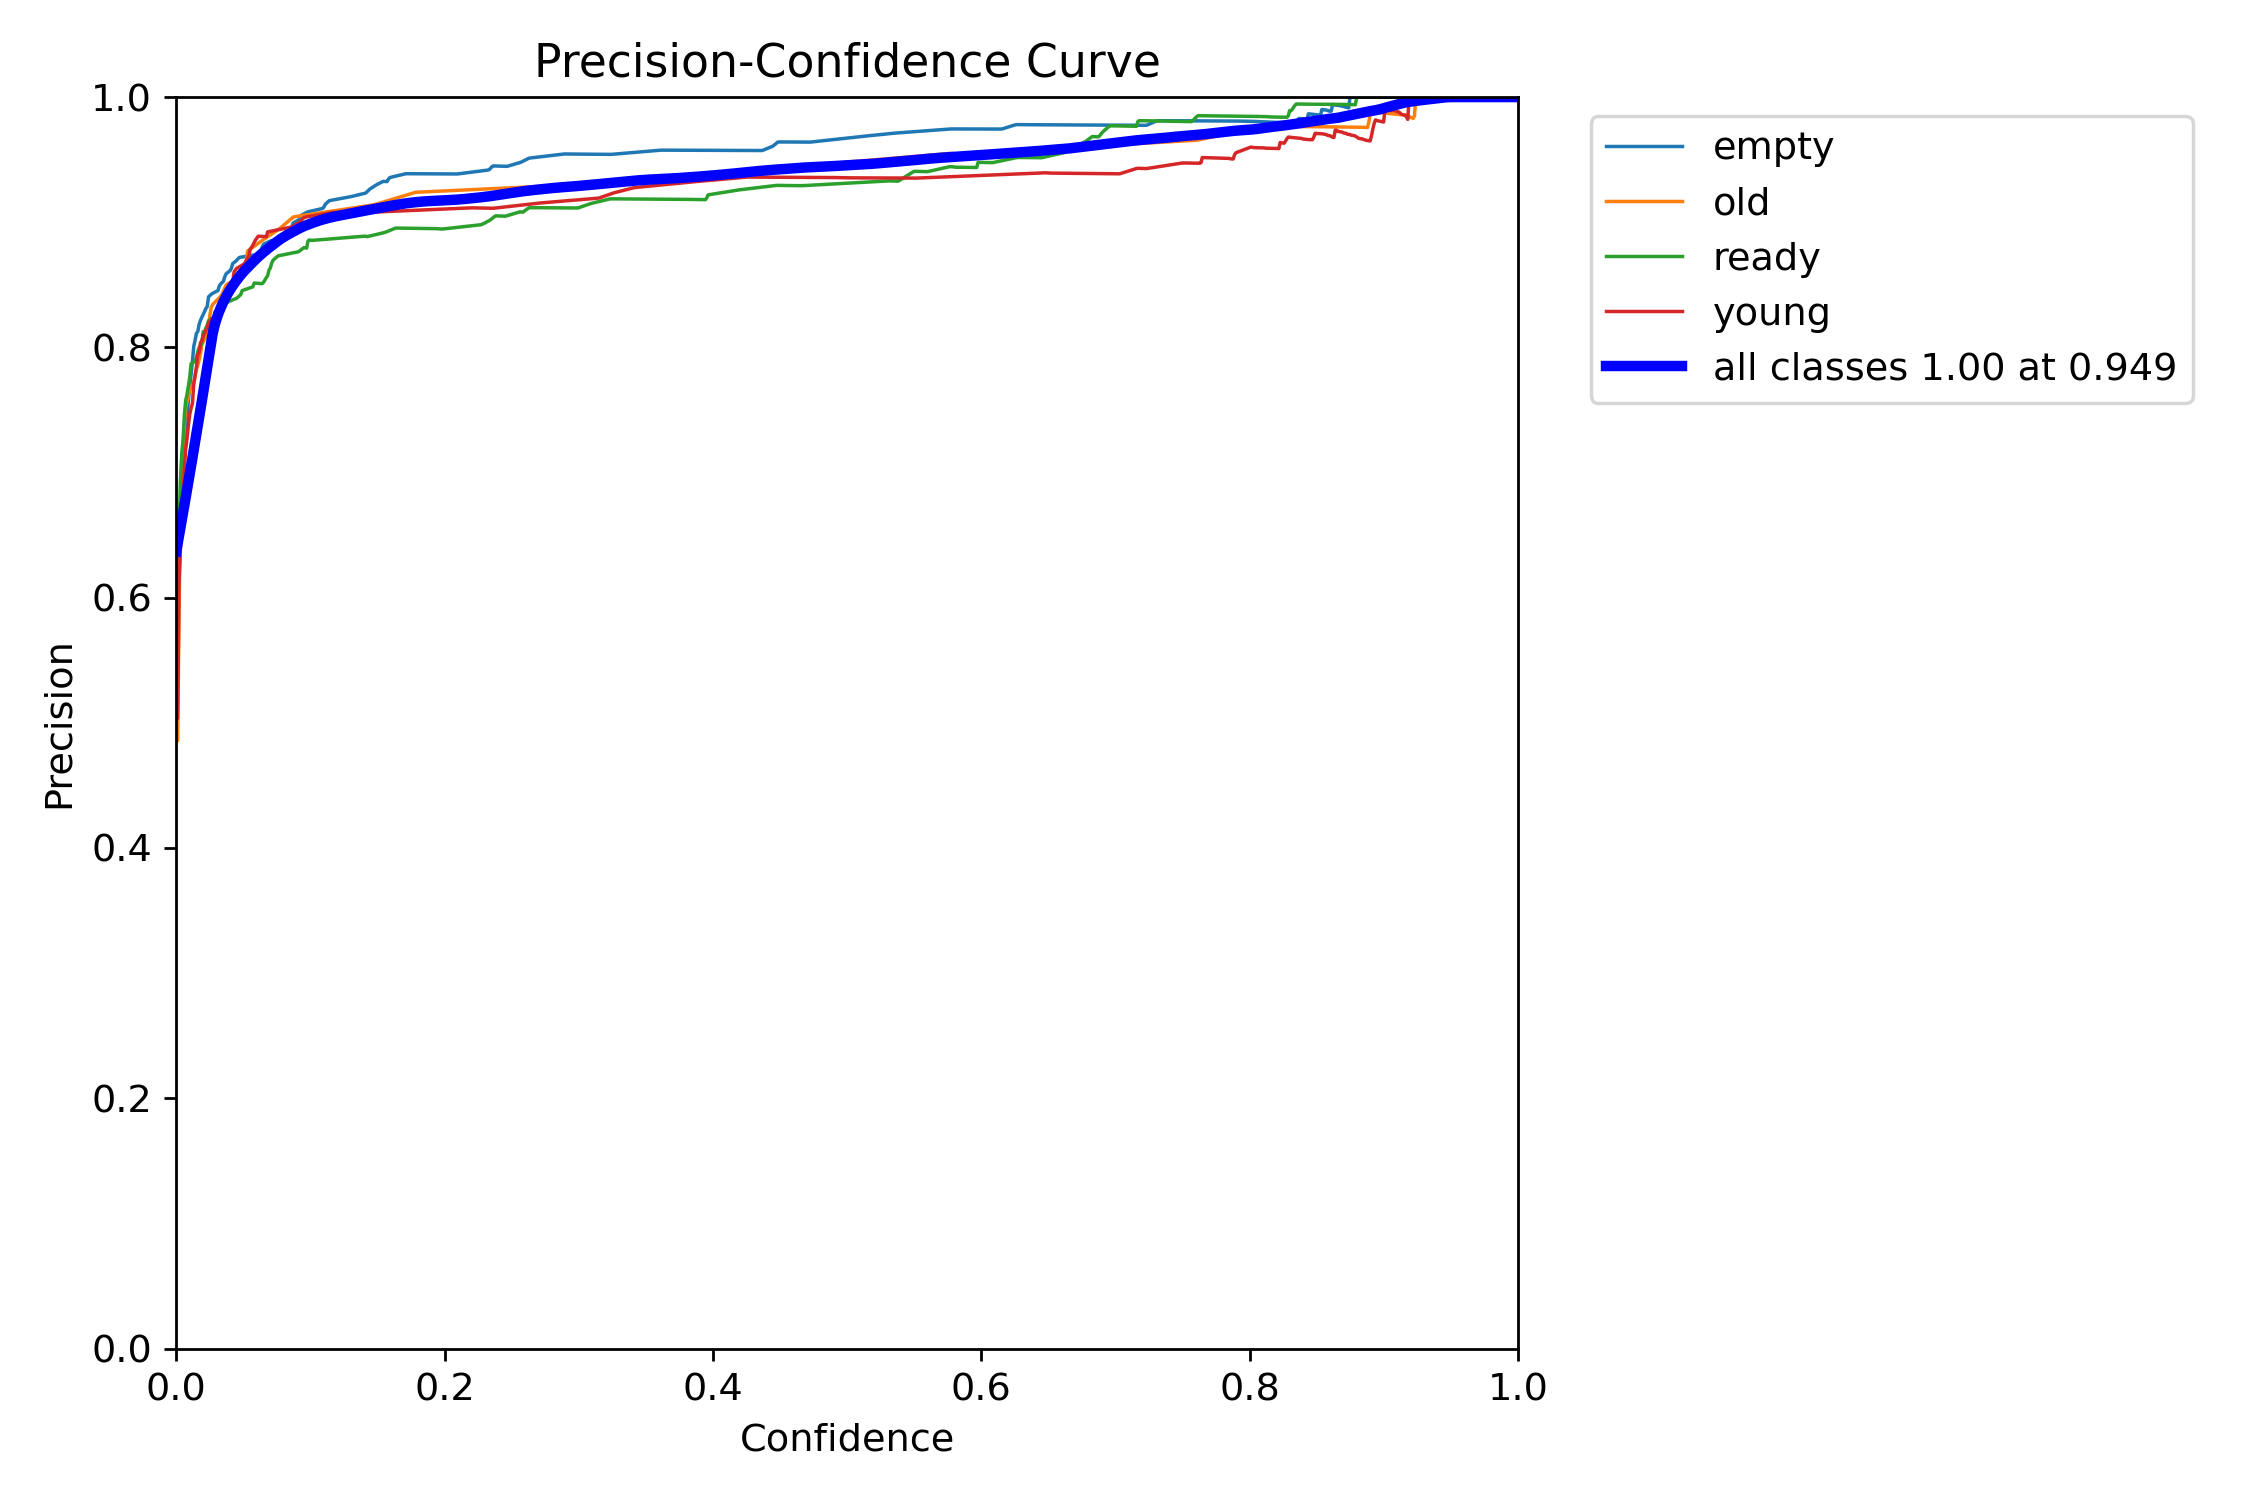
\includegraphics[width=0.95\linewidth]{images/P_curve.png}
    \caption{Đường cong Precision}
    \label{fig:training-result-p}

    \end{subfigure}%
    \begin{subfigure}{.5\textwidth}
        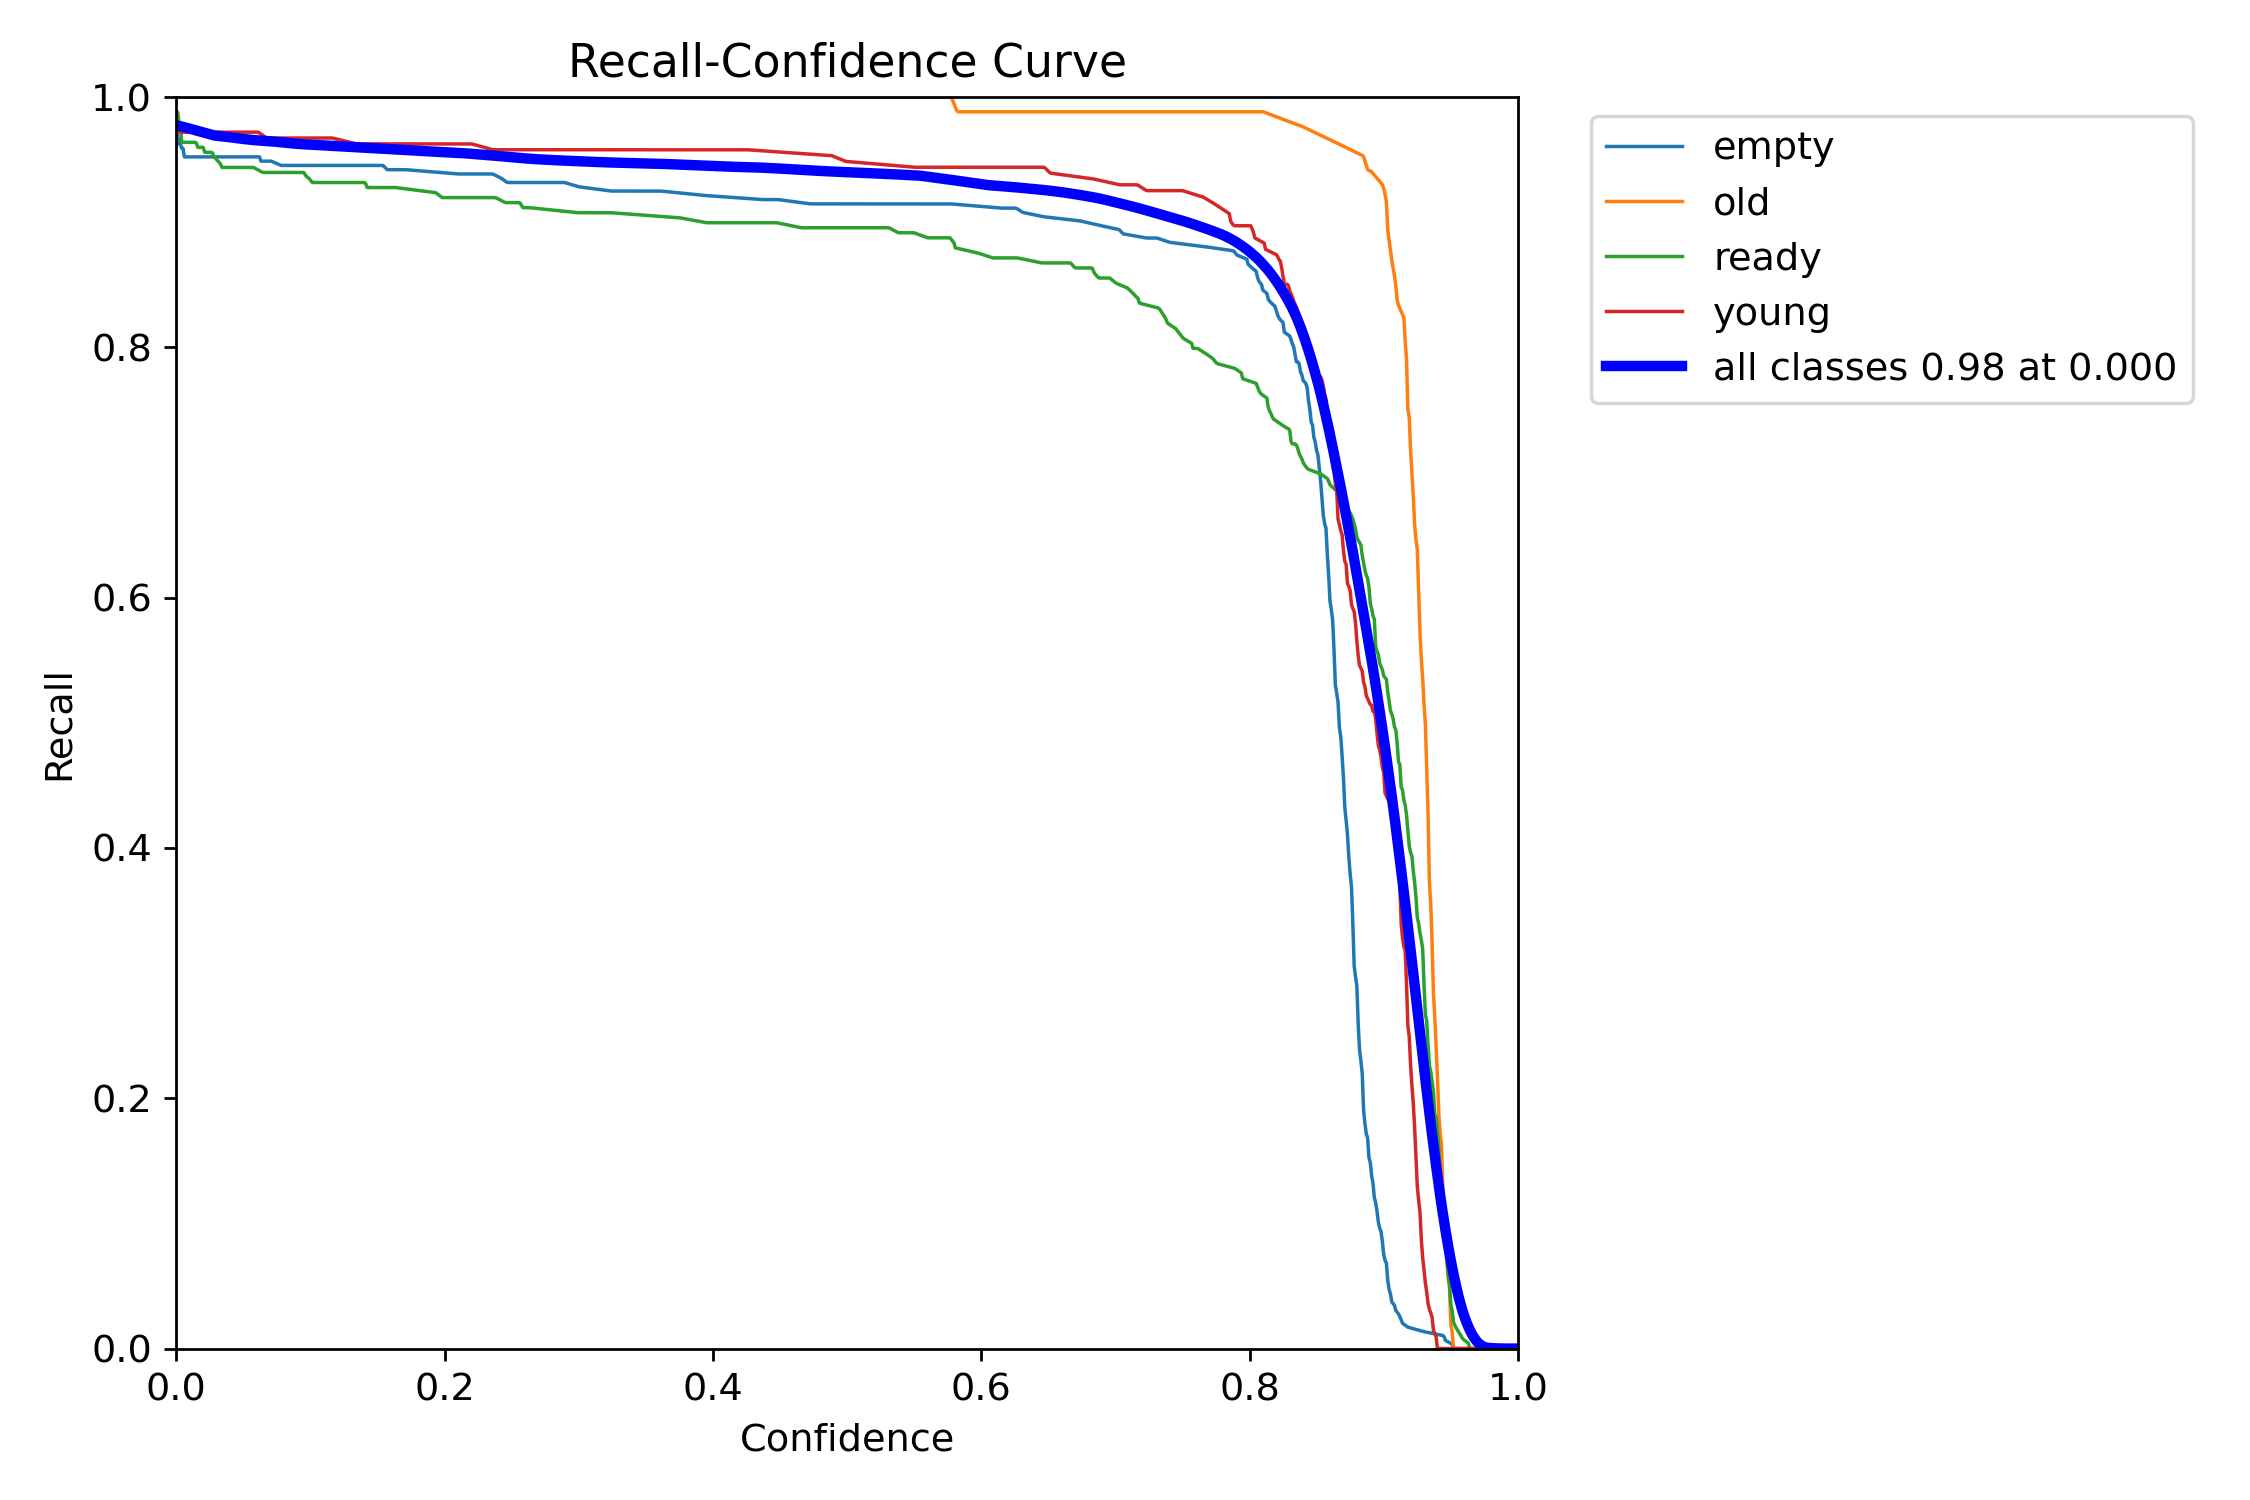
\includegraphics[width=0.95\linewidth]{images/R_curve.png}
    \caption{Đường cong Recall}
    \label{fig:training-result-r}
    \end{subfigure}
    \begin{subfigure}{.5\textwidth}
        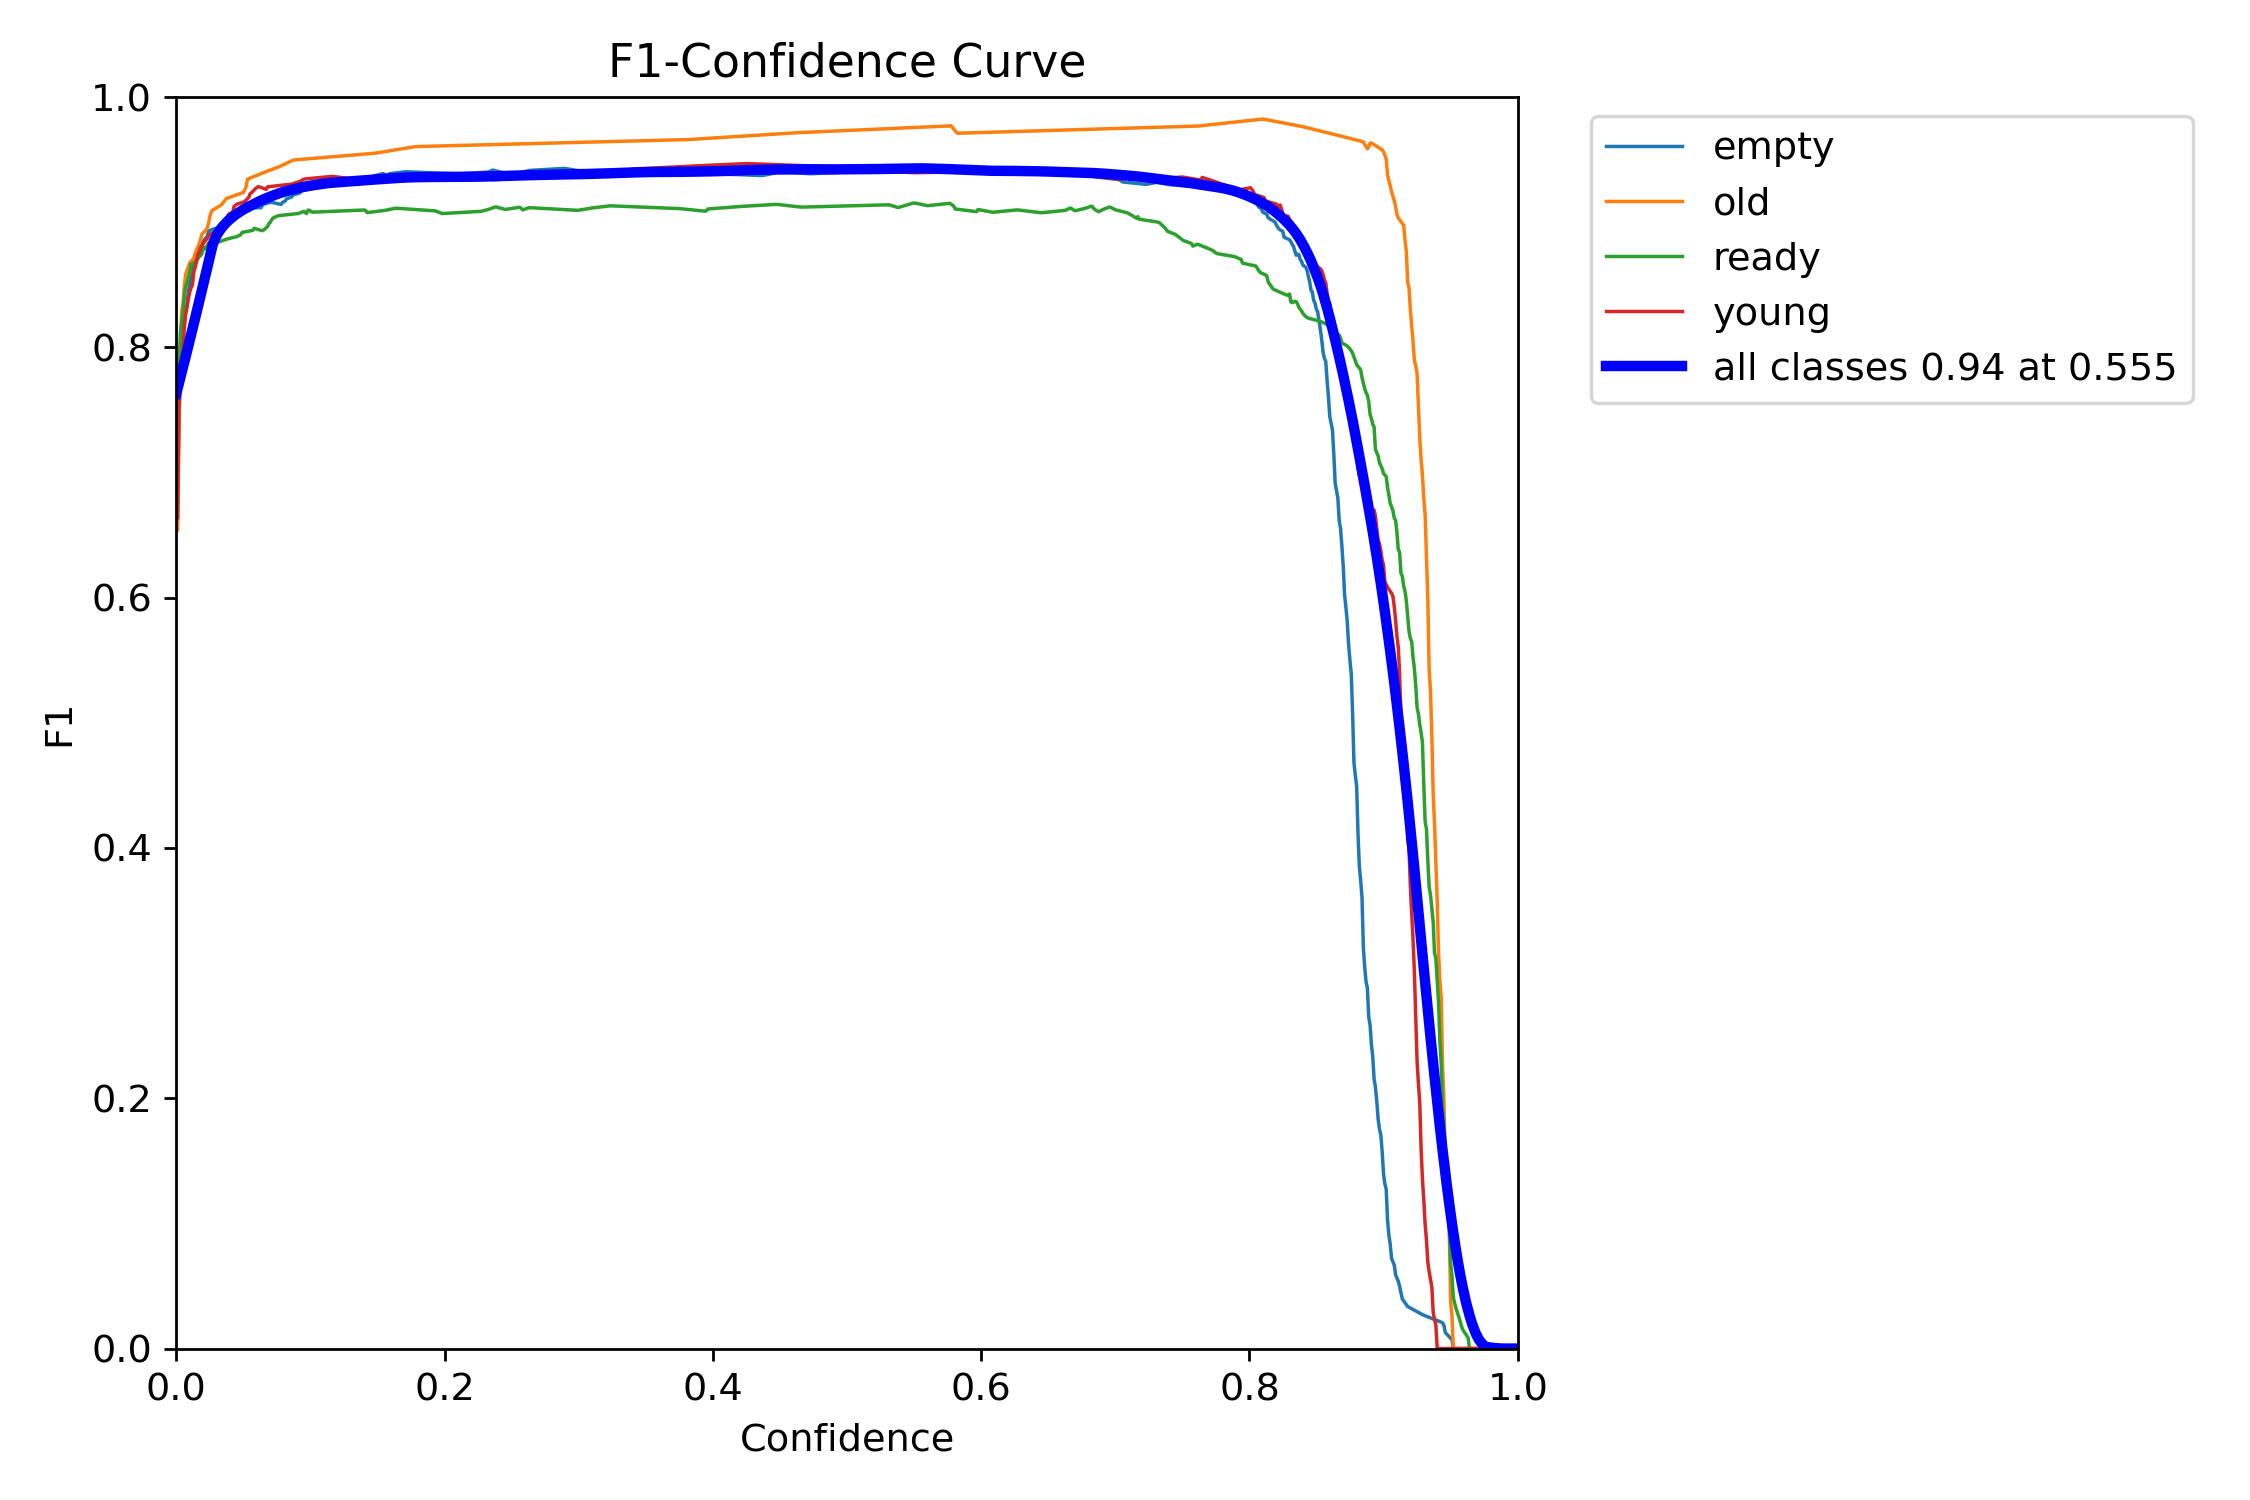
\includegraphics[width=0.95\linewidth]{images/F1_curve.png}
    \caption{Đường cong F1-score}
    \label{fig:training-result-f1}

    \end{subfigure}
    \caption{Kết quả huấn luyện}

    \label{fig:training-result}
\end{figure}

\begin{figure}[h]
    \centering
    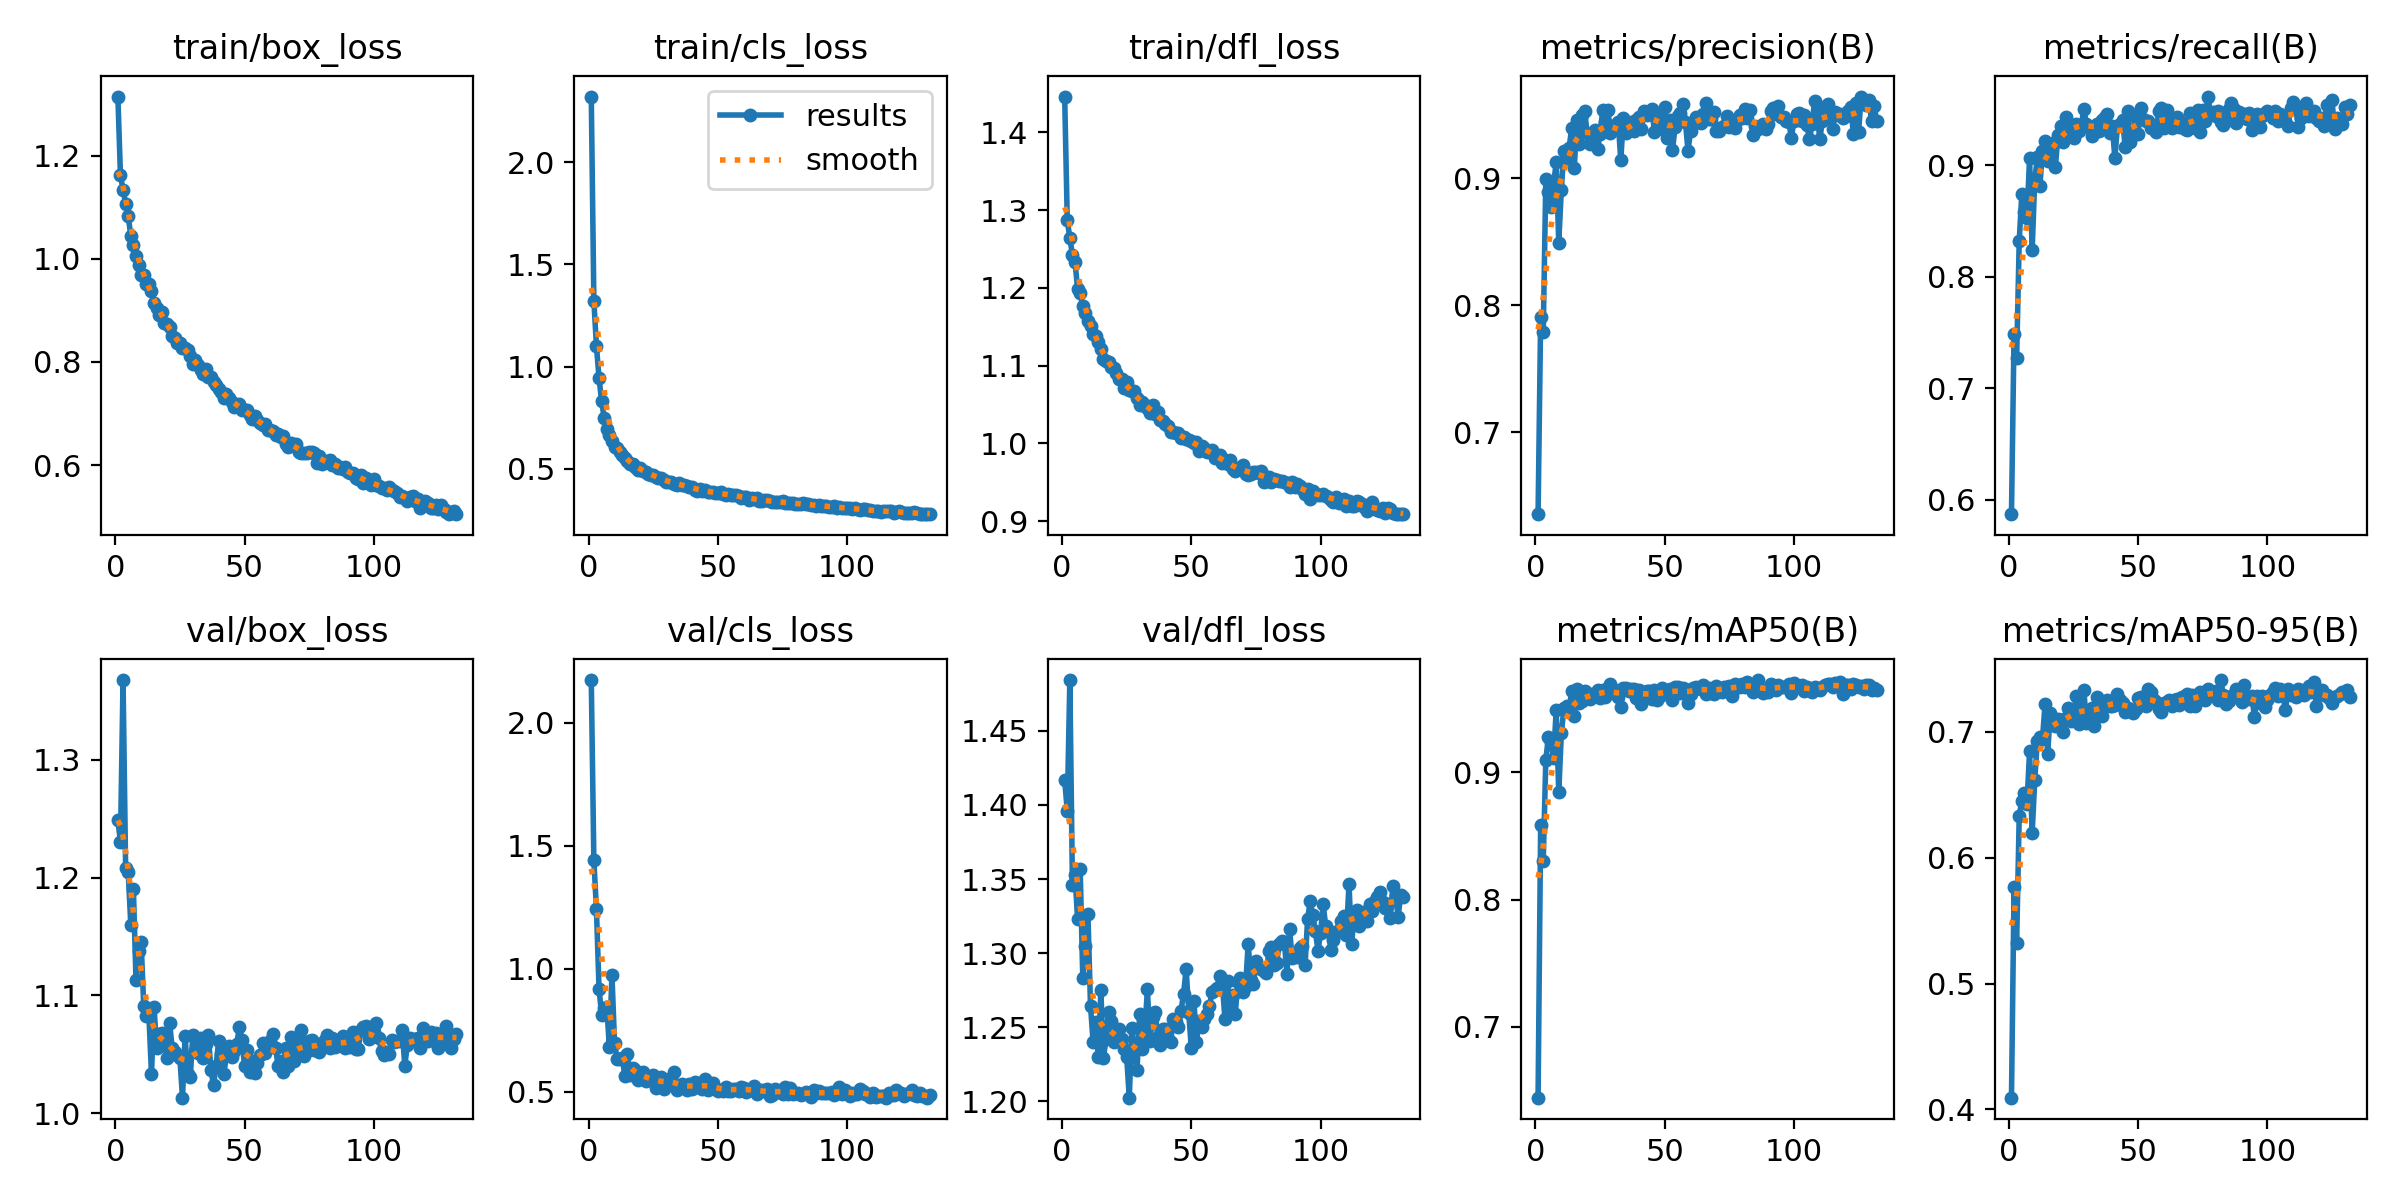
\includegraphics[width=0.85\linewidth]{images/results.png}
    \caption{Đồ thị mất mát}
    \label{fig:loss}
\end{figure}

Đồ thị \ref{fig:loss} cho thấy số lượng dữ liệu huấn luyện nhỏ nên gặp nhiều nhiều đỉnh trong đồ thị. Đồ thị mất mát cho việc phát hiện lớp "cls\_loss" có độ mịn, luôn ở ngưỡng thấp nên hoàn toàn phù hợp cho phát hiện trạng thái phát triển của nấm.

Đồ thị hàm mất mát cho hộp bao còn không ổn định, nhiều đỉnh cũng như gợn sóng. Điều này có thể nhận biết thông qua việc phát hiện hộp bao nhỏ hơn hoặc lớn hơn vật thể trong ảnh. Tuy nhiên, đối với bài toán phát hiện trạng thái phát triển của nấm, vị trí và kích thước hộp bao không cần độ chính xác tuyệt đối, vì vậy, mô hình huấn luyện này cũng phù hợp cho việc phát hiện trạng thái phát triển của nấm.

\begin{figure}[H]
	\centering
	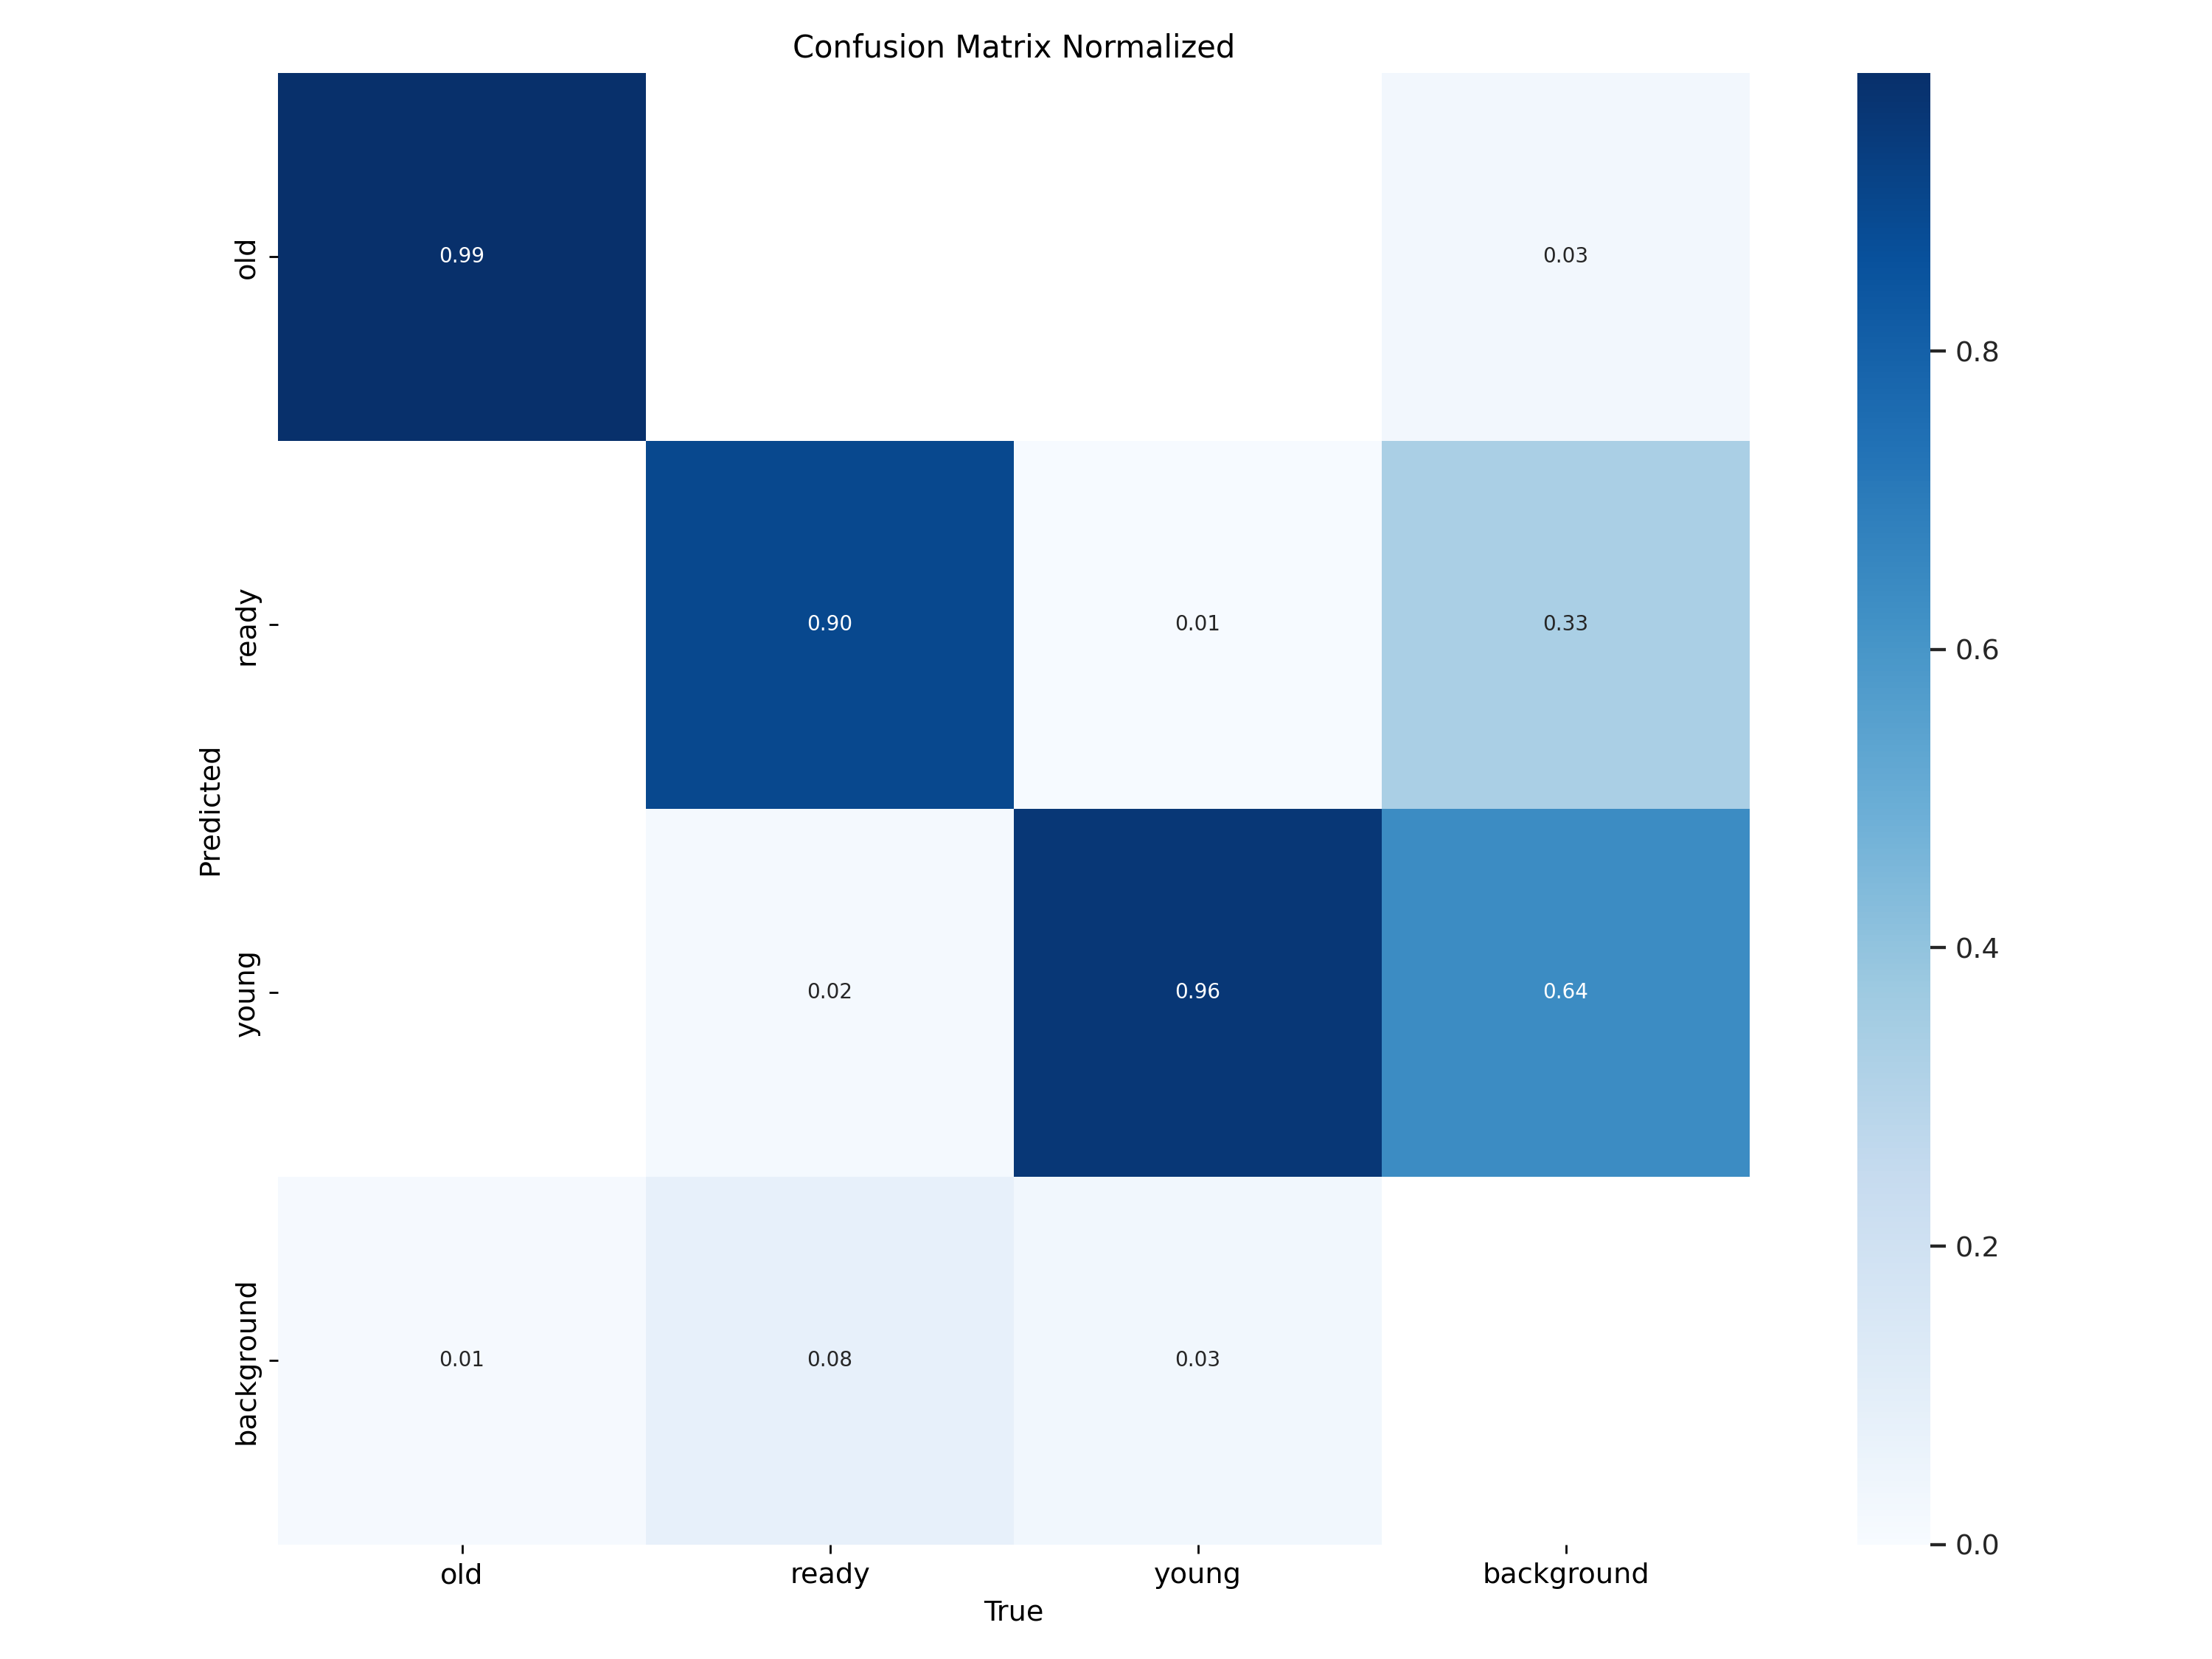
\includegraphics[width=0.8\linewidth]{images/confusion_matrix_normalized.png}
	\caption{Ma trận nhầm lẫn}
	\label{fig:confusion-matrix}
\end{figure}

Ma trận nhầm lẫn trong hình \ref{fig:confusion-matrix} cho thấy mô hình suy đoán chính xác ở mức cao, tuy nhiên nhiều trường hợp không suy đoán được trạng thái của nấm do tập dữ liệu còn nhỏ, chư bao quát hết các trường hợp trong quá trình huấn luyện. Vì vậy, tập dữ liệu cần bổ sung thêm.

\section{Tích hợp hệ thống}

\begin{figure}[h]
	\centering
	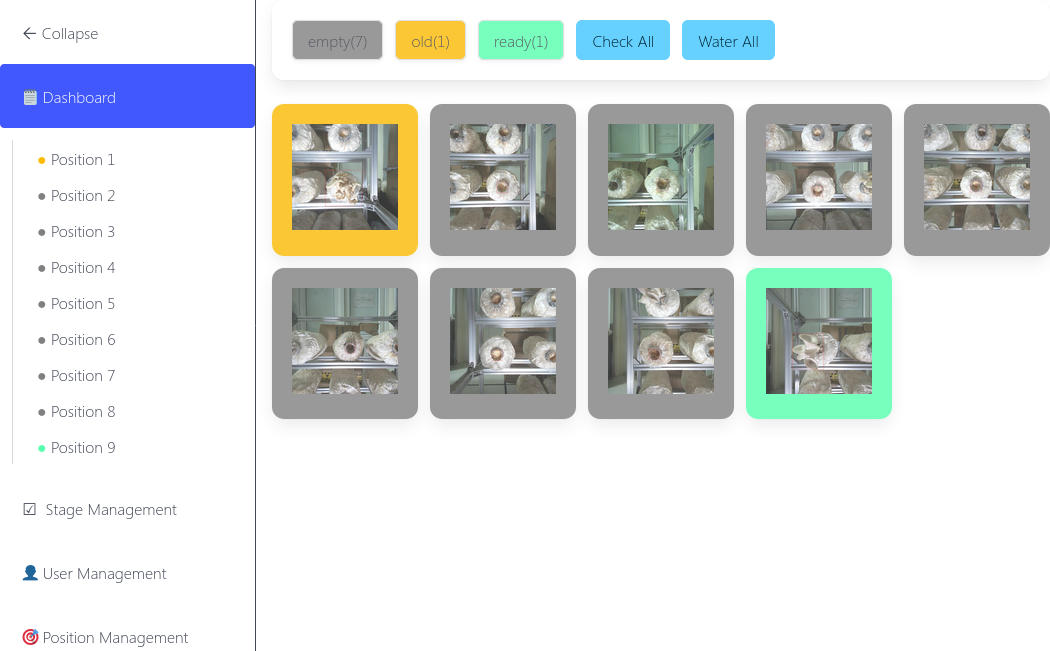
\includegraphics[width=0.8\linewidth]{images/ui-dashboard}
	\caption{Giao diện bảng điều khiển}
	\label{fig:ui-dashboard}
\end{figure}

\begin{figure}[H]
	\centering
	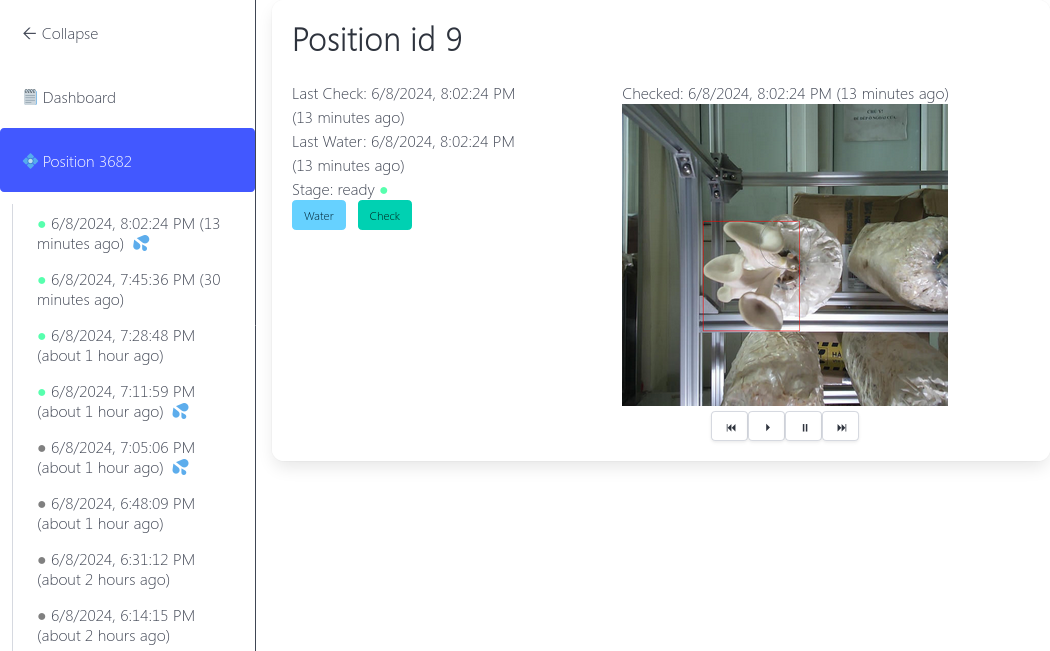
\includegraphics[width=0.8\linewidth]{images/ui-detail}
	\caption{Giao diện xem chi tiết vị trí}
	\label{fig:ui-detail}
\end{figure}

Sau khi huấn luyện, mô hình có thể được sử dụng trong hệ thống điều khiển. Giao diện người dùng hiển thị trạng thái hệ thống, hiển thị hình ảnh theo dõi và kết quả dự đoán trạng thái sinh trưởng chính xác. Màu của mỗi ô tương ứng với từng trạng thái sinh trưởng trống, non, trưởng thành, giá là xám, trắng, xanh lá, vàng như hình \ref{fig:ui-dashboard}.

Trong giao diện hiển thị chi tiết vị trí nấm, các trạng thái sinh trưởng cùng thời điểm chụp ảnh cũng được hiển thị rõ ràng. Ngoài ra, người dùng có thể xem lại quá trình sinh trưởng của nấm theo trình tự thời gian như hình \ref{fig:ui-detail}.

Qua thời gian thử nghiệm và tinh chỉnh, hệ thống có thể đưa ra kết quả kiểm tra tương đối chính xác cho từng vị trí nấm để có thể tưới nước theo từng giai đoạn phát triển của nấm. Các chức năng phụ như xem lại quá trình phát triển của nấm hoạt động đúng theo phương hướng đề ra. Tuy nhiên, một số ít thời điểm hệ thống không suy đoán được loại nấm tại vị trí chỉ định.

\section{Tổng kết chương}

Trong nửa đầu chương 3, đồ án mô tả các hoạt động của hệ thống sử dụng sơ đồ usecase, sơ đồ đối tượng và sơ đồ hợp tác mô tả hoạt động của người dùng với hệ thống, cấu trúc bên trong của hệ thống và hoạt động của các thành phần đó.

Tiếp theo, đồ án mô tả quá trình xây dựng tập dữ liệu huấn luyện và huấn luyện bao gồm:
\begin{itemize}
    \item Thu thập dữ liệu từ các nguồn khác nhau để đảm bảo độ đa dạng và đủ lớn cho quá trình huấn luyện.
    \item Tiền xử lý và chuẩn bị dữ liệu huấn luyện để đảm bảo chất lượng và độ tin cậy của dữ liệu.
    \item Huấn luyện mô hình và đánh giá hiệu suất của nó để đảm bảo rằng mô hình có khả năng phân loại các loại nấm một cách chính xác.
\end{itemize}

Cuối cùng, mô hình thị giác máy tính được tích hợp và chạy thử trong hệ thống với thành công bước đầu khi nhận diện trạng thái sinh trưởng của nấm thành công.